\documentclass[11pt,a4paper]{article}
\usepackage[utf8]{inputenc}
\usepackage[T1]{fontenc}
\usepackage[brazil]{babel}
\usepackage{lmodern}
\usepackage[margin=2.5cm]{geometry}
\usepackage{amsmath,amssymb,bm}
\usepackage{booktabs,tabularx,multirow,longtable,array}
\usepackage{graphicx}
\usepackage{xcolor}
\usepackage{float}
\usepackage{algorithm}
\usepackage[noend]{algpseudocode}
\usepackage[numbers,sort&compress]{natbib}
\usepackage{microtype}
\usepackage[most]{tcolorbox}
\usepackage{titlesec,fancyhdr,enumitem}
\usepackage[font=small,labelfont={bf,color=azul},labelsep=period,justification=justified]{caption}
\usepackage[colorlinks,linkcolor=azul,citecolor=azul,urlcolor=azul]{hyperref}
\usepackage{url}
\usepackage{setspace}
\setstretch{1.25}

% ------------------------------------------------------------------ estilo
\definecolor{azul}{RGB}{20,70,140}
\definecolor{azulclaro}{RGB}{235,242,252}
\definecolor{areia}{RGB}{252,247,232}
\definecolor{ocre}{RGB}{170,120,20}
\titleformat{\section}{\Large\sffamily\bfseries\color{azul}}{\thesection}{0.8em}{}[{\color{azul}\titlerule[0.6pt]}]
\titleformat{\subsection}{\large\sffamily\bfseries\color{azul}}{\thesubsection}{0.8em}{}
\titleformat{\subsubsection}{\normalsize\sffamily\bfseries}{\thesubsubsection}{0.8em}{}
\titlespacing*{\section}{0pt}{2.2ex plus .5ex}{1.2ex}
\titlespacing*{\subsection}{0pt}{1.8ex plus .5ex}{0.8ex}
\setlist{itemsep=2pt,topsep=4pt}
\pagestyle{fancy}
\fancyhf{}
\fancyhead[L]{\small\sffamily\color{azul}Alocação de interceptadores contra enxames mistos}
\fancyhead[R]{\small\sffamily\thepage}
\renewcommand{\headrulewidth}{0.4pt}
\setlength{\headheight}{14pt}

% cartao de metodo (secao 4) e quadro de conceito (revisao)
\newtcolorbox{metodo}[1]{breakable,enhanced,colback=azulclaro,colframe=azul,boxrule=0.6pt,arc=2pt,
  left=6pt,right=6pt,top=4pt,bottom=4pt,fonttitle=\sffamily\bfseries,title={#1},before skip=8pt,after skip=8pt}
\newtcolorbox{conceitobox}[1]{breakable,enhanced,colback=areia,colframe=ocre,boxrule=0.5pt,arc=2pt,
  left=6pt,right=6pt,top=3pt,bottom=3pt,fonttitle=\sffamily\bfseries\small,title={Conceito: #1},fontupper=\small,
  before skip=6pt,after skip=6pt}

\newcommand{\todo}[1]{\textcolor{red}{[\textbf{A FAZER:} #1]}}
\newcommand{\inp}[1]{\IfFileExists{#1.tex}{\input{#1}}{\todo{tabela \texttt{\detokenize{#1}} será gerada pelos scripts de análise}}}
\newcommand{\orig}{\par\smallskip\noindent\textbf{Origem.}~}
\newcommand{\ideia}{\par\smallskip\noindent\textbf{Ideia.}~}
\newcommand{\func}{\par\smallskip\noindent\textbf{Como funciona.}~}
\newcommand{\prop}{\par\smallskip\noindent\textbf{Propriedades.}~}
\newcommand{\adap}{\par\smallskip\noindent\textbf{Adaptações.}~}
\newcommand{\parm}{\par\smallskip\noindent\textbf{Parâmetros.}~}
\newcommand{\espera}{\par\smallskip\noindent\textbf{O que esperar.}~}
\newcommand{\conceito}[1]{\textbf{#1}}
\floatname{algorithm}{Algoritmo}
\renewcommand{\algorithmicrequire}{\textbf{Entrada:}}
\renewcommand{\algorithmicensure}{\textbf{Saída:}}
\DeclareMathOperator*{\argmin}{arg\,min}
\DeclareMathOperator*{\argmax}{arg\,max}


\begin{document}
\thispagestyle{empty}
\begin{center}
{\color{azul}\rule{\textwidth}{1.2pt}}\\[10pt]
{\sffamily\bfseries\LARGE\color{azul}Alocação de interceptadores contra enxames mistos\\[2pt]
de drones e iscas sob informação de radar}\\[8pt]
{\sffamily\large Revisão de técnicas e avaliação comparativa reprodutível}\\[8pt]
{\color{azul}\rule{\textwidth}{1.2pt}}\\[14pt]
{\large Otávio Zordan Alves}\\[18pt]
\end{center}
\begin{abstract}
Ataques com dezenas a centenas de aeronaves não tripuladas baratas, lançadas em ondas e misturadas a iscas, tornaram-se
frequentes na última década. Contra eles, o recurso que se esgota primeiro não é o sensor nem o efetor, e sim a
capacidade de \emph{decidir}: qual interceptador lançar contra qual ameaça, quando lançar, quando guardar e quando trocar
de alvo. Essa decisão é estudada há mais de sessenta anos como problema de atribuição arma--alvo (WTA), mas a literatura
recente se dividiu em comunidades que raramente se comparam entre si --- pesquisa operacional, robótica multiagente,
controle preditivo e aprendizado por reforço ---, cada uma com seu próprio simulador e suas próprias hipóteses. Este
artigo faz três coisas. Primeiro, formula o problema como um processo de decisão parcialmente observável, em que o
decisor vê apenas pistas de radar ruidosas e possivelmente falsas, não distingue drones armados de iscas e paga tanto
pelos impactos quanto pelos interceptadores desperdiçados. Segundo, revisa as técnicas de alocação em oito famílias,
explicando a ideia, a origem e as hipóteses de cada uma. Terceiro, \emph{implementa e compara todas as técnicas
revisadas} --- 23 algoritmos de alocação e 6 políticas aprendidas --- num mesmo simulador aberto, com relevo real, rede
de radares com difração, ruído, vieses e falsos alarmes e rastreador IMM. O conjunto de avaliação tem 192 missões em
seis cidades brasileiras (São José dos Campos, Taubaté, Itajubá, São Paulo, Rio de Janeiro e Brasília): enxames de 12 a
48 vetores que misturam quatro classes de ameaça com parâmetros de fontes abertas --- drones de ataque de longo alcance,
iscas, munições vagantes e FPV ---, atacando ativos reais de infraestrutura extraídos do OpenStreetMap, por rotas
planejadas sobre o relevo e com chegada coordenada, contra uma defesa montada sem conhecimento do ataque. Duas cidades
(Rio de Janeiro e Brasília) ficam reservadas para teste, o que permite medir desempenho, custo computacional e
generalização com testes estatísticos pareados.
\todo{resumo dos resultados quantitativos quando os experimentos terminarem.}
\end{abstract}

\noindent\textbf{Palavras-chave:} atribuição arma--alvo; enxames de drones; iscas; alocação de tarefas; leilão;
consenso; metaheurísticas; aprendizado por reforço; rastreamento por radar; infraestrutura crítica.

\tableofcontents
\newpage
% =====================================================================================================
\section{Introdução}\label{sec:intro}

\subsection{O problema em uma frase}
Um conjunto de aeronaves hostis se aproxima de uma região a ser defendida. O defensor dispõe de um conjunto de
\emph{interceptadores} --- pequenas aeronaves capazes de alcançar e neutralizar uma ameaça --- distribuídos em bases, e
de uma rede de radares que detecta as ameaças. A cada instante, o defensor precisa decidir \emph{quais interceptadores
lançar, contra quais ameaças e quando}, sabendo que cada interceptador só pode ser usado uma vez e que as ameaças
mais perigosas são as que se dirigem às áreas mais importantes. Este artigo trata dessa decisão, que chamamos de
\emph{alocação de interceptadores}.

\subsection{Origem histórica: o problema de atribuição arma--alvo}
A pergunta ``quais armas devem engajar quais alvos?'' é um dos problemas mais antigos da pesquisa operacional, a
disciplina que aplica modelos matemáticos a decisões de alocação de recursos. Ela foi formalizada no fim da década de
1950, no contexto da defesa contra bombardeiros e mísseis, como o problema de \conceito{atribuição arma--alvo}
(\emph{weapon--target assignment}, WTA)~\cite{manne1958}. Na forma clássica, há um conjunto de armas e um conjunto de
alvos; cada alvo tem um \emph{valor} (quanto dano causa se sobreviver) e cada par arma--alvo tem uma
\emph{probabilidade de abate} (a chance de aquela arma destruir aquele alvo). Quer-se escolher qual arma vai contra qual
alvo de modo a minimizar o valor esperado dos alvos que sobrevivem.

Um exemplo mínimo dá a intuição. Suponha dois alvos, um de valor 10 e outro de valor 1, e duas armas, cada uma com
probabilidade 0,8 de destruir qualquer alvo. Mandar uma arma contra cada alvo deixa sobreviver, em média,
$10\times0{,}2+1\times0{,}2=2{,}2$. Mandar as duas contra o alvo valioso deixa sobreviver
$10\times0{,}2\times0{,}2+1=1{,}4$, porque o alvo de valor 10 só sobrevive se as duas armas falharem. A melhor decisão
depende, portanto, dos valores e das probabilidades, e não é óbvia mesmo em instâncias pequenas.

Nos anos seguintes surgiram as primeiras heurísticas --- regras práticas que dão boas soluções sem garantia de serem as
melhores ---, como o \emph{máximo retorno marginal}, que designa uma arma de cada vez ao alvo em que ela mais reduz o
valor sobrevivente~\cite{denbroeder1959}. Na década de 1980, a defesa contra mísseis balísticos motivou a versão
\conceito{dinâmica} do problema, em que os engajamentos ocorrem em estágios e o defensor observa o resultado de um
estágio antes de decidir o próximo~\cite{hosein1990}. Na mesma época, provou-se que o WTA é \conceito{NP-completo}: não
se conhece algoritmo que o resolva exatamente em tempo que cresça só polinomialmente com o número de armas e
alvos~\cite{lloyd1986}, o que, na prática, significa que instâncias grandes só podem ser resolvidas aproximadamente.
Três revisões consolidaram a área: \citet{cai2006} sobre a versão dinâmica, \citet{roux2007} sobre sistemas de avaliação
de ameaças e atribuição de armas (TEWA, na sigla em inglês) e \citet{kline2019} sobre formulações e algoritmos exatos e
heurísticos.

\subsection{O problema hoje: enxames baratos que chegam em ondas}
Na última década, o problema mudou de escala e de natureza. Aeronaves não tripuladas baratas permitem ao atacante
lançar dezenas a centenas de vetores de uma vez, e a defesa tradicional, baseada em poucos mísseis caros, deixa de ser
economicamente viável: não faz sentido gastar um míssil de alto custo contra um drone que custa uma pequena fração dele.
Alguns casos ilustram a progressão:
\begin{itemize}
  \item Em janeiro de 2018, treze pequenos drones de construção rudimentar atacaram a base aérea russa de Khmeimim e o
        ponto naval de Tartus, na Síria; segundo o relato russo, foram neutralizados por guerra eletrônica e defesa
        antiaérea~\cite{bellingcat2018}. Foi um dos primeiros ataques amplamente noticiados com vários drones
        coordenados.
  \item Em setembro de 2019, o ataque às instalações de petróleo de Abqaiq e Khurais, na Arábia Saudita, combinou 18
        drones e cerca de sete mísseis de cruzeiro e interrompeu temporariamente cerca de metade da produção saudita, com
        a defesa praticamente sem engajar~\cite{idsa2019}. Mostrou que poucas dezenas de vetores baratos podem causar dano
        estratégico.
  \item Em abril de 2024, o ataque iraniano contra Israel empregou mais de 300 vetores --- cerca de 170 drones, mais de
        30 mísseis de cruzeiro e mais de 120 balísticos ---, e, segundo as forças israelenses, 99\,\% foram interceptados por
        uma defesa multinacional coordenada~\cite{pbs2024}. Nesse caso, a coordenação de muitos efetores contra muitas
        ameaças foi o fator decisivo.
  \item Na guerra na Ucrânia, ataques noturnos com centenas de drones do tipo Shahed levaram, a partir de 2024--2025, ao
        uso em massa de \emph{drones interceptadores}: aeronaves baratas lançadas contra as ameaças a partir das
        indicações do radar~\cite{pravda2025}.
\end{itemize}
O último caso é exatamente o cenário deste artigo: muitos interceptadores baratos e \emph{descartáveis} (cada um
neutraliza uma única ameaça e é consumido), despachados a partir de um quadro de radar comum contra muitas ameaças que
chegam em \conceito{ondas} --- grupos sucessivos, separados por alguns minutos, que tentam \conceito{saturar} a defesa,
isto é, apresentar mais ameaças simultâneas do que ela consegue tratar. Nesse regime, a qualidade da \emph{alocação}
decide quantas ameaças passam: a mesma frota de interceptadores, mal distribuída, deixa passar ameaças que uma
distribuição melhor teria detido.

\subsection{Por que a alocação é difícil}
Três fatores tornam a decisão difícil.
\begin{enumerate}
  \item \textbf{Explosão combinatória.} Com 48 ameaças e 60 interceptadores, o número de maneiras de designar
        interceptadores a ameaças é astronômico (maior que $10^{60}$), e a decisão precisa ser tomada em fração de
        segundo e refeita continuamente.
  \item \textbf{Informação imperfeita.} O defensor não vê as aeronaves; vê \conceito{pistas de radar}. Uma pista é a
        estimativa, produzida por um algoritmo de rastreamento a partir das medidas dos radares, da posição e da
        velocidade de algo que se move. Essa estimativa tem erro; não traz a identidade da aeronave; desaparece quando a
        aeronave se esconde atrás do relevo; e pode ser um \conceito{falso alarme} --- uma pista que não corresponde a
        aeronave nenhuma, criada por ruído ou por reflexos do terreno. Nos nossos cenários, a maioria das pistas pode ser
        falsa.
  \item \textbf{Ameaças heterogêneas e iscas.} Um ataque real mistura vetores muito diferentes: drones de ataque de
        longo alcance, rápidos e de rota pré-programada; munições vagantes, que orbitam o alvo antes de mergulhar; drones
        FPV, lentos, rentes ao solo e pilotados, capazes de manobrar; e \conceito{iscas}, aeronaves baratas sem carga
        explosiva, com assinatura de radar parecida, lançadas para atrair interceptadores. Parte das ameaças voa baixo
        para se esconder do radar no relevo. Quase todos os métodos de alocação estimam onde a ameaça estará supondo que
        ela mantém a velocidade atual, e nenhum tem como saber se uma pista é um drone armado ou uma isca --- e cada
        interceptador gasto numa isca é um a menos para a próxima ameaça real.
\end{enumerate}

\subsection{Lacunas da literatura}
A literatura recente oferece muitas propostas, mas três lacunas impedem saber qual usar:
\begin{enumerate}
  \item \textbf{Hipóteses otimistas.} A maior parte da literatura de WTA supõe alvos conhecidos e probabilidades de abate
        dadas; trabalhos de robótica e controle supõem consciência situacional perfeita e ameaças em linha reta ou com
        velocidade constante. Nenhuma dessas hipóteses vale contra um enxame misto, com iscas, visto por radar.
  \item \textbf{Escala pequena e cenários abstratos.} Os trabalhos brasileiros mais próximos, do Instituto Tecnológico
        de Aeronáutica~\cite{ricardo2023,feitosa2025,afonso2020,cruz2025}, modelam com cuidado a dinâmica dos defensores,
        mas usam de 3 a 6 ameaças. Em geral, os cenários da literatura são sintéticos: alvos e rotas sorteados, e radares
        posicionados sabendo de onde o ataque virá.
  \item \textbf{Comparações incomparáveis.} Os trabalhos de aprendizado por reforço~\cite{liu2023drones,palmas2025,jia2026}
        e de contra-enxame~\cite{strickland2018} usam simuladores, métricas e linhas de base próprios --- muitas vezes uma
        só linha de base. Não é possível saber, a partir da literatura, se uma política aprendida supera o método húngaro,
        ou se uma árvore de comportamento supera um leilão.
\end{enumerate}

\subsection{Contribuições e organização}
Este artigo contribui com:
\begin{itemize}
  \item uma \textbf{formulação} do problema como processo de decisão parcialmente observável, decomposta em avaliação de
        ameaças, alocação e guiagem, que explicita o que cada família de métodos supõe sobre a informação e sobre o alvo
        (Seção~\ref{sec:problema});
  \item uma \textbf{revisão} das técnicas de alocação em oito famílias, da pesquisa operacional ao aprendizado por
        reforço, explicando a ideia de cada uma e comparando os trabalhos mais próximos (Seção~\ref{sec:revisao});
  \item a \textbf{implementação de todas as técnicas revisadas} numa interface comum --- 29 métodos, cada um descrito por
        origem, funcionamento, adaptações e parâmetros ---, com a verificação de que as implementações reproduzem as
        equivalências teóricas conhecidas (Seção~\ref{sec:metodos});
  \item um \textbf{conjunto de missões realistas} e aberto: 192 missões em seis cidades brasileiras, com enxames de até
        48 vetores que misturam drones de ataque de longo alcance, iscas, munições vagantes e FPV (parâmetros de fontes
        abertas), atacando ativos reais de infraestrutura do OpenStreetMap por rotas planejadas sobre o relevo, contra
        uma defesa montada sem conhecer o ataque (Seção~\ref{sec:dataset});
  \item uma \textbf{avaliação reprodutível} num simulador aberto (Seção~\ref{sec:ambiente}), com divisão treino/teste
        por cidade, sementes pareadas e testes estatísticos, que mede tanto o dano quanto o desperdício de
        interceptadores (Seções~\ref{sec:protocolo} e~\ref{sec:resultados}).
\end{itemize}
A Seção~\ref{sec:discussao} discute os resultados, as limitações e as recomendações.

% =====================================================================================================
\section{Formulação do problema}\label{sec:problema}

Esta seção descreve o cenário, escreve o problema de decisão em linguagem matemática, explica por que ele não pode ser
resolvido exatamente, mostra como os métodos práticos o decompõem e define as grandezas que quase todos os métodos usam.

\subsection{Cenário}
Uma região contém \conceito{zonas prioritárias} $\mathcal{Z}$ --- círculos que representam ativos importantes, como uma
base, uma usina ou uma subestação --- e \conceito{bases de interceptadores}, de onde partem os defensores. Um conjunto
$\mathcal{A}$ de $N$ ameaças entra na região em ondas e segue rotas que terminam num \conceito{ponto de impacto}, onde a
ameaça mergulha contra o alvo. Cada ameaça pertence a uma \conceito{classe} --- drone de ataque de longo alcance,
munição vagante, drone FPV ou \conceito{isca} --- que determina a sua velocidade, altura, manobra e o \conceito{valor de
dano} $\nu_a$ da sua carga: $\nu_a=1$, $0{,}5$ e $0{,}25$ para as três classes armadas e $\nu_a=0$ para a isca, que não
carrega explosivo e existe só para atrair interceptadores. Se uma ameaça chega ao impacto sem ser interceptada, causa um
dano $w_a=\nu_a\,w_P$, com $w_P=10$, se o impacto é dentro de uma zona prioritária, e $w_a=\nu_a\,w_O$, com $w_O=1$, fora
dela; a razão de 10 para 1 expressa que proteger os ativos defendidos é muito mais valioso que evitar impactos em ativos
secundários.

O defensor tem $M\ge N$ interceptadores. Cada um voa a velocidade $v_d$, tem autonomia $T_d$ (tempo máximo de voo) e um
\conceito{sensor próprio} de curto alcance $r_s$: enquanto está longe da ameaça, o interceptador depende das pistas de radar
para saber para onde ir; quando chega a menos de $r_s$, passa a ver a ameaça diretamente. Um interceptador neutraliza a
ameaça quando passa a menos de $r_c$ dela (\conceito{contato}) e é consumido nesse contato. Um interceptador que é
lançado e não neutraliza uma ameaça armada --- porque esgota a autonomia sem contato, porque abate uma isca ou porque
ainda voa sem uso quando o ataque termina --- é \conceito{desperdiçado}: foi gasto sem proteger nada. A
Tabela~\ref{tab:notacao} resume a notação.

\begin{table}[t]
\centering
\caption{Notação principal.}
\label{tab:notacao}
\small
\begin{tabularx}{\textwidth}{@{}lX@{}}
\toprule
Símbolo & Significado \\
\midrule
$\mathcal{A}$, $N$; $\mathcal{D}$, $M$ & aeronaves e seu número; interceptadores e seu número \\
$\nu_a$; $w_a$; $w_P=10$, $w_O=1$ & valor de dano da classe (isca: 0); dano da ameaça $a$; peso dentro e fora de zona prioritária \\
$W$, $\eta=0{,}2$ & interceptadores desperdiçados num episódio; penalidade por desperdício \\
$v_d$, $T_d$, $r_s$, $r_c$ & velocidade, autonomia, alcance do sensor e raio de contato do interceptador \\
$\mathcal{P}(t)=\{p_j\}$ & quadro de radar: pistas com posição $\bm{x}_j$, velocidade $\bm{v}_j$, incerteza, idade \\
$\mathcal{D}_t$ & fila de interceptadores que decidem na rodada $t$ \\
$x_{ij}\in\{0,1\}$ & designação do interceptador $i$ à pista $j$ (1 se designado) \\
$t^\star_{ij}$, $c_{ij}$ & tempo previsto de interceptação; custo com histerese (E2) \\
$w_j$, $t^Z_j$ & peso de prioridade e tempo até a zona inferidos da pista (E3) \\
$q_{ij}$, $V_j$, $S_j$ & probabilidade de sucesso, valor e sobrevivência da pista (E4) \\
$F(\bm{x})$ & valor esperado destruído numa rodada \eqref{eq:F} \\
$D$, $C$ & dano normalizado \eqref{eq:dano} e custo \eqref{eq:custo_ep} de um episódio \\
\bottomrule
\end{tabularx}
\end{table}

\subsection{O que o defensor observa}
O defensor não vê as aeronaves. A cada instante ele recebe o \conceito{quadro de radar} $\mathcal{P}(t)$, a lista de
pistas mantida pelo rastreador. Cada pista $p_j$ traz uma posição estimada $\bm{x}_j$, uma velocidade estimada $\bm{v}_j$,
uma medida da incerteza dessas estimativas, a idade (há quanto tempo foi atualizada) e o número de medidas que a
sustentam. Três coisas \emph{não} são observadas e precisam ser inferidas ou ignoradas: (i) qual aeronave uma pista
representa, ou se representa alguma (pode ser falso alarme); (ii) o ponto de impacto e, portanto, se a ameaça vai cair
numa zona prioritária; e (iii) a classe da ameaça --- em particular, se é uma isca, que voa como as demais e tem
assinatura de radar parecida. Além disso, ameaças escondidas pelo relevo simplesmente não aparecem no quadro.

\subsection{Formulação como processo de decisão parcialmente observável}
Um \conceito{processo de decisão de Markov} (MDP) descreve um sistema que evolui no tempo sob as ações de um decisor: em
cada instante o sistema está num \emph{estado}; o decisor escolhe uma \emph{ação}; o sistema passa a um novo estado de
forma possivelmente aleatória (a \emph{transição}), e isso gera um custo ou uma recompensa. ``De Markov'' significa que o
próximo estado depende só do estado e da ação atuais, e não de todo o passado. Quando o decisor não vê o estado, mas
apenas uma \emph{observação} parcial e ruidosa dele, o processo é \conceito{parcialmente observável} (POMDP). Nesse caso, a
melhor decisão depende de todo o histórico de observações, porque é desse histórico que o decisor infere o estado. Uma
\conceito{política} é a regra que associa a cada histórico uma ação, e resolver o problema é encontrar a política de menor
custo esperado.

O nosso problema é um POMDP com decisões a cada $\Delta_d=2$~s (as \conceito{rodadas de decisão}):
\begin{itemize}
  \item \textbf{Estado} $s_t$: posição, velocidade, rota, classe e situação (viva, interceptada ou caída) de cada
        ameaça; posição, autonomia restante, alvo e situação (na base, em voo ou consumido) de cada interceptador; e o
        estado interno do rastreador.
  \item \textbf{Observação} $o_t$: o quadro de radar $\mathcal{P}(t)$, o estado dos próprios interceptadores e as zonas
        prioritárias.
  \item \textbf{Ação} $a_t$: em cada rodada decide a \conceito{fila} $\mathcal{D}_t$, formada pelos interceptadores ociosos
        nas bases e pelos interceptadores em voo cuja reavaliação venceu. Cada um recebe uma pista ou a \emph{ação nula}
        (esperar na base ou manter o alvo atual). A ação é uma matriz binária $\bm{x}$, com $x_{ij}=1$ se o interceptador
        $i$ é designado à pista $j$, sujeita a
        \begin{equation}
          \sum_j x_{ij}\le1\quad\forall i,\qquad \sum_i x_{ij}+n_j^0\le\bar n\quad\forall j .
          \label{eq:restr}
        \end{equation}
        A primeira restrição diz que cada interceptador persegue no máximo uma pista; a segunda, que cada pista recebe no
        máximo $\bar n$ interceptadores, contando os $n_j^0$ que já a perseguem ($\bar n=1$ por padrão).
  \item \textbf{Transição}: as ameaças avançam pelas rotas (as FPV manobram e algumas reagem ao interceptador); os interceptadores em trânsito voam
        em direção ao ponto previsto de encontro com a sua pista e, ao entrar no alcance do sensor, passam a perseguir a
        aeronave diretamente; os radares medem e o rastreador atualiza as pistas. Há contato quando um interceptador passa
        a menos de $r_c$ de uma aeronave, e impacto quando uma aeronave chega ao fim da rota.
  \item \textbf{Objetivo}: minimizar o valor esperado do \conceito{dano normalizado},
        \begin{equation}
          \min_{\pi}\ \mathbb{E}_\pi[D],\qquad
          D = \frac{\sum_{a\in\mathcal{A}} w_a\,\mathbf{1}\{a\text{ atinge o impacto}\}}{\sum_{a\in\mathcal{A}} w_a}\in[0,1],
          \label{eq:dano}
        \end{equation}
        em que $\mathbf{1}\{\cdot\}$ vale 1 se a condição é verdadeira e 0 caso contrário. $D$ é a fração do dano possível
        que de fato ocorreu: vale 0 se todas as ameaças armadas foram interceptadas e 1 se nenhuma foi. A normalização
        permite comparar cenários com números diferentes de ameaças. As iscas não entram em~\eqref{eq:dano}, porque
        $w_a=0$, mas pesam no \conceito{custo}, que soma ao dano a penalidade dos interceptadores desperdiçados:
        \begin{equation}
          C = \frac{\sum_{a\in\mathcal{A}} w_a\,\mathbf{1}\{a\text{ atinge o impacto}\} + \eta\,W}{\sum_{a\in\mathcal{A}} w_a},
          \qquad \eta=0{,}2 .
          \label{eq:custo_ep}
        \end{equation}
        Um interceptador desperdiçado custa um quinto do impacto de uma ameaça plena num ativo não defendido. Com
        $\eta=0$, $C=D$; com $\eta>0$, um método que dispara contra tudo o que aparece --- e, portanto, contra as iscas ---
        é penalizado mesmo que não deixe passar nada. Reportamos as duas grandezas: $D$ mede a proteção, e $C$, a
        proteção descontado o gasto.
\end{itemize}

\paragraph{Por que não resolver o POMDP diretamente.} Resolver exatamente um POMDP exige raciocinar sobre a distribuição
de probabilidade de todos os estados possíveis, o que só é viável em problemas minúsculos. Aqui, o estado é contínuo e de
alta dimensão (posições e velocidades de dezenas de aeronaves e interceptadores), o espaço de ações é combinatório (as
designações possíveis entre dezenas de interceptadores e pistas) e a classe e o comportamento de cada ameaça não são
conhecidos pelo defensor. Todos os métodos práticos, inclusive os aprendidos, recorrem a aproximações: decompõem o
problema e resolvem cada parte com informação local.

\subsection{Decomposição em camadas}
A decisão completa se decompõe naturalmente em três camadas, que correspondem às comunidades da literatura:
\begin{enumerate}
  \item \textbf{Avaliação de ameaças}: decidir quais pistas são aeronaves reais, quão perigosas são e quanto tempo há até
        que causem dano.
  \item \textbf{Alocação}: dada essa avaliação, decidir qual interceptador vai contra qual pista nesta rodada, quais ficam
        esperando e quais trocam de alvo.
  \item \textbf{Guiagem}: dado o alvo, levar o interceptador até ele.
\end{enumerate}
Este artigo compara técnicas da camada de \emph{alocação}. As outras duas são mantidas fixas e iguais para todos os
métodos: a avaliação de ameaças é uma regra física comum, descrita abaixo, ou um classificador aprendido (nas redes
neurais); a guiagem é uma lei fixa, escolhida por um experimento separado (Seção~\ref{sec:res_guiagem}). Fixar as outras
camadas garante que as diferenças medidas venham da alocação.

\subsection{Relação com o WTA clássico}
Se considerarmos uma única rodada, a alocação é uma instância do WTA estático~\cite{manne1958}: designar armas $i$ a alvos
$j$ de valor $V_j$, com probabilidade de abate $q_{ij}$, minimizando o valor esperado que sobrevive,
\begin{equation}
  \min_{x}\ \sum_{j} V_j \prod_{i} (1-q_{ij})^{x_{ij}}\quad\text{s.a. \eqref{eq:restr}}.
  \label{eq:wta}
\end{equation}
A leitura é direta: $(1-q_{ij})$ é a chance de a arma $i$ falhar contra o alvo $j$; o expoente $x_{ij}$ faz o fator
aparecer só se a arma foi designada; o produto sobre $i$ é, portanto, a chance de \emph{todas} as armas designadas a $j$
falharem, isto é, de $j$ sobreviver; multiplicada pelo valor $V_j$ e somada sobre os alvos, dá o valor sobrevivente
esperado. O produto é o que torna o problema não linear e difícil.

O nosso problema difere do WTA clássico em três pontos. É \emph{dinâmico}: a alocação se repete a cada rodada e pode
ser revista, como no WTA dinâmico~\cite{hosein1990}. É \emph{parcialmente observável}: alocam-se pistas, que podem ser
falsas ou estar erradas, e não alvos conhecidos. E é \emph{acoplado à cinemática}: a probabilidade de sucesso $q_{ij}$
não é dada, e depende de quanto tempo o interceptador leva para chegar e de como o alvo manobra. No caso particular em que
cada alvo recebe no máximo um interceptador e todas as probabilidades são próximas de 1, o produto em~\eqref{eq:wta}
desaparece, e o problema se torna um \emph{problema de atribuição linear}, que pode ser resolvido exatamente e
rapidamente~\cite{kuhn1955} (Seção~\ref{sec:met_atrib}).

\subsection{Elementos comuns a todos os métodos}\label{sec:comuns}
Quatro grandezas, calculadas apenas a partir das observações, são usadas por quase todos os métodos. Definimo-las aqui
uma única vez; os métodos da Seção~\ref{sec:metodos} se referem a elas como (E1) a (E4).

\paragraph{(E1) Filtro de plausibilidade.} Se cada pista recebesse um interceptador, os falsos alarmes consumiriam boa
parte da frota. A forma mais simples de \emph{avaliação de ameaças} é uma regra física: as classes de ameaça conhecidas
voam dentro de um envelope de velocidade, razão de subida e altura; uma pista fora desse envelope provavelmente é falsa.
O envelope precisa cobrir todas as classes, inclusive o mergulho final, e por isso é largo. Os métodos só consideram
pistas com
\begin{equation}
  \Pi(p_j)=\mathbf{1}\{12\le\|\bm{v}_{j}^{h}\|\le75\}\;\mathbf{1}\{|v_{j}^{z}|\le60\}\;\mathbf{1}\{-50\le h_j^{\mathrm{AGL}}\le2500\}=1,
  \label{eq:plaus}
\end{equation}
em que $\bm{v}_j^h$ é a velocidade horizontal estimada (m/s), $v_j^z$ a vertical (m/s) e $h_j^{\mathrm{AGL}}$ a altura
sobre o terreno (m). Os falsos alarmes do modelo de radar tendem a ter velocidades incoerentes, porque resultam de
associações espúrias entre medidas; uma aeronave que manobra forte pode, por sua vez, ser momentaneamente rejeitada, que
é o custo dessa regra. Note que o filtro separa aeronaves de falsos alarmes, mas não separa iscas de drones armados:
uma isca é uma aeronave e passa no filtro. As redes neurais trocam~\eqref{eq:plaus} por um classificador aprendido.

\paragraph{(E2) Custo de interceptação e histerese.} A grandeza física central da alocação é o tempo que um interceptador
leva para alcançar uma pista. Se o interceptador $i$ está em $\bm{x}_i$ e a pista $j$ está em $\bm{x}_j$ com velocidade
$\bm{v}_j$, e supondo que a pista mantém essa velocidade, o encontro ocorre no instante $t$ em que a distância percorrida
pelo interceptador, $v_d\,t$, iguala a distância até a posição futura da pista, $\|\bm{x}_j+\bm{v}_jt-\bm{x}_i\|$. Elevando
ao quadrado, $t$ é a menor raiz positiva de
\begin{equation}
  (\|\bm{v}_j\|^2-v_d^2)\,t^2+2\,(\bm{r}_{ij}\!\cdot\!\bm{v}_j)\,t+\|\bm{r}_{ij}\|^2=0,\qquad \bm{r}_{ij}=\bm{x}_j-\bm{x}_i,
  \label{eq:tint}
\end{equation}
que chamamos de \conceito{tempo previsto de interceptação} $t^\star_{ij}$. Essa previsão supõe \emph{velocidade
constante}: é exatamente a hipótese que uma manobra evasiva viola, e o erro aparece como pistas que ``fogem'' do ponto
previsto. O custo usado pelos métodos é
\begin{equation}
  c_{ij} = \begin{cases} \kappa^{\mathbf{1}\{j=j_i\}}\,t^\star_{ij}, & t^\star_{ij}\le T_d-\tau_i,\\ \infty, & \text{caso contrário,}\end{cases}
  \label{eq:custo}
\end{equation}
em que $\tau_i$ é o tempo que o interceptador já voou: se o encontro exigir mais autonomia do que resta, o par é
inviável (custo infinito). O fator $\kappa=0{,}7$ é uma \conceito{histerese}, termo que designa a tendência de um sistema
de permanecer no estado em que está. Para um interceptador já em voo, a sua pista atual $j_i$ entra com custo
multiplicado por 0,7, como se estivesse 30\,\% mais perto. Assim, ele só troca de alvo se a alternativa for claramente
melhor. Sem histerese, duas pistas a distâncias parecidas, cujas estimativas oscilam com o ruído do radar, fariam o
interceptador trocar de alvo a cada rodada e não chegar a nenhum. Por exemplo, se a pista atual está a 50~s e outra a
40~s, o custo atual é $0{,}7\times50=35<40$, e o interceptador mantém o alvo; se a outra estiver a 30~s, ele troca.

\paragraph{(E3) Peso de prioridade e tempo até a zona.} O defensor não sabe onde cada aeronave vai cair, mas pode inferir
a prioridade pela geometria da pista em relação às zonas. Sejam $d_j$ a distância da pista à borda da zona prioritária
mais próxima (negativa se já está dentro) e $\dot d_j$ a velocidade com que ela se aproxima do centro dessa zona. Definimos
o \conceito{peso de prioridade} e o \conceito{tempo até a zona}
\begin{equation}
  w_j=\begin{cases} w_P, & d_j\le 0,\\ (w_P+w_O)/2, & \dot d_j>5\text{ m/s e } d_j<3\text{ km},\\ w_O, & \text{caso contrário;}\end{cases}
  \qquad
  t^Z_j=\begin{cases}0, & d_j\le0,\\ d_j/\dot d_j, & \dot d_j>1\text{ m/s},\\ \infty,&\text{caso contrário.}\end{cases}
  \label{eq:peso}
\end{equation}
Uma pista dentro de uma zona recebe o peso máximo; uma pista fora, mas que se aproxima depressa de uma zona próxima,
recebe um peso intermediário; as demais, o peso mínimo. O tempo até a zona é a distância dividida pela velocidade de
aproximação, e é infinito para pistas que não se aproximam. Rotas planejadas sobre o relevo, que passam perto de ativos
que não são o seu alvo (Seção~\ref{sec:dataset}), enganam exatamente essa inferência.

\paragraph{(E4) Modelo de sucesso e objetivo de valor esperado.} Os métodos derivados do WTA precisam de uma
probabilidade de sucesso $q_{ij}$, que o problema não fornece. Estimamo-la por
\begin{equation}
  q_{ij} = P_T\,e^{-c_{ij}/\tau_q}\,\mathbf{1}\{c_{ij}<\infty\},\qquad P_T=0{,}85,\ \tau_q=600\text{ s}.
  \label{eq:q}
\end{equation}
O fator $P_T$ é a chance de contato quando o interceptador chega perto do alvo, medida no experimento de guiagem
(Seção~\ref{sec:res_guiagem}). O fator exponencial reduz essa chance para trânsitos longos, porque quanto mais tempo o
interceptador voa guiado pelo radar, mais a pista envelhece, mais o alvo pode manobrar ou sair da cobertura. Com esses
valores, um encontro a 30~s tem $q\approx0{,}81$, e um a 300~s tem $q\approx0{,}52$.

Cada pista tem valor $V_j=w_j$. Se já há interceptadores em voo contra a pista $j$ (o conjunto $\mathcal{F}_j$, que não
decide nesta rodada), a chance de ela ainda sobreviver é $S_j=\prod_{k\in\mathcal{F}_j}(1-q_{kj})$, a
\conceito{sobrevivência atual}. O objetivo de uma rodada é o \conceito{valor esperado destruído},
\begin{equation}
  F(\bm{x}) = \underbrace{\sum_j V_j S_j\Big[1-\prod_{i}(1-q_{ij})^{x_{ij}}\Big]}_{\text{valor esperado destruído}}
  - \underbrace{\sum_{i}\ell_i\sum_j x_{ij}}_{\text{custo de lançamento}}
  - \underbrace{M\sum_j\max\!\Big(0,\ n_j^0+\sum_i x_{ij}-\bar n\Big)}_{\text{penalidade de capacidade}} .
  \label{eq:F}
\end{equation}
O primeiro termo é~\eqref{eq:wta} reescrito como ganho: para cada pista, o valor ainda em risco ($V_jS_j$) vezes a
chance de que pelo menos um dos novos interceptadores acerte. O segundo termo cobra $\ell_i=0{,}05$ por interceptador
lançado da base (zero para os que já estão em voo). Sem esse custo, como cada lançamento sempre aumenta um pouco o
primeiro termo, o ótimo seria lançar todos os interceptadores contra qualquer pista, sem guardar nenhum para as ondas
seguintes. O valor 0,05 corresponde a 5\,\% do valor de uma pista comum: só se lança se a chance de ganho compensar. O
terceiro termo impõe a restrição de capacidade~\eqref{eq:restr} como penalidade ($M=10$), forma conveniente para os
métodos de busca, que podem então explorar soluções inviáveis sem quebrar.

% =====================================================================================================
\section{Revisão da literatura}\label{sec:revisao}

\subsection{Como a revisão foi feita}
Esta é uma revisão narrativa estruturada: em vez de enumerar exaustivamente todos os trabalhos publicados, ela organiza a
literatura em famílias de técnicas, explica a ideia de cada família e seleciona os trabalhos que a definiram ou que mais
se aproximam do nosso problema. A busca usou Google Scholar, IEEE Xplore, ScienceDirect e arXiv, com combinações dos termos
\emph{weapon--target assignment}, \emph{dynamic weapon--target assignment}, \emph{threat evaluation and weapon assignment},
\emph{counter-UAV}, \emph{counter-swarm}, \emph{interceptor allocation}, \emph{task allocation}, \emph{auction},
\emph{consensus}, \emph{behavior tree} e \emph{reinforcement learning}, complementada pelas referências dos trabalhos
encontrados e por trabalhos brasileiros recentes do Instituto Tecnológico de Aeronáutica. Os critérios de seleção foram:
(i) propor ou consolidar uma técnica de alocação usada na prática ou em pesquisa; (ii) tratar defesa contra múltiplas
ameaças aéreas; ou (iii) servir de linha de base comum na área. A Tabela~\ref{tab:linha_tempo} situa os marcos no tempo.

\begin{table}[t]
\centering
\caption{Linha do tempo dos marcos revisados.}
\label{tab:linha_tempo}
\small
\begin{tabularx}{\textwidth}{@{}l X l@{}}
\toprule
Ano & Marco & Ref. \\
\midrule
1955--1957 & Método húngaro para o problema de atribuição & \cite{kuhn1955,munkres1957} \\
1958--1959 & Formulação do WTA e heurística de máximo retorno marginal & \cite{manne1958,denbroeder1959} \\
1960 & Modelos de detecção de alvos com seção radar flutuante & \cite{swerling1960} \\
1986 & Prova de que o WTA é NP-completo & \cite{lloyd1986} \\
1988 & Algoritmo de leilão; filtro IMM para rastreamento & \cite{bertsekas1988,blom1988} \\
1990 & WTA dinâmico e \emph{shoot--look--shoot} & \cite{hosein1990} \\
2002--2003 & Colônia de formigas e algoritmo genético com sementes gulosas para o WTA & \cite{lee2002aco,lee2003ga} \\
2004 & Taxonomia da alocação de tarefas em robótica multiagente & \cite{gerkey2004} \\
2006--2007 & Revisões do WTA dinâmico e de sistemas TEWA; solução exata e VLSN para o WTA & \cite{cai2006,roux2007,ahuja2007} \\
2009 & Leilões por consenso (CBAA/CBBA) & \cite{choi2009} \\
2011 & Imitação iterativa (DAgger) & \cite{ross2011} \\
2017 & PPO; DeepSets; Transformer & \cite{schulman2017,zaheer2017,vaswani2017} \\
2018 & Contra-enxame contra ataques de saturação & \cite{strickland2018} \\
2019 & Revisão do WTA; atenção para problemas combinatórios & \cite{kline2019,kool2019} \\
2020 & Alocação e trajetória por MILP de horizonte deslizante & \cite{afonso2020} \\
2023 & Reforço para alocação em enxames; árvores de comportamento contra kamikazes & \cite{liu2023drones,ricardo2023} \\
2025--2026 & Reforço para priorização de interceptações; árvore com utilidade; MIQP contra ameaças aéreas; atenção em grafos + MAPPO & \cite{palmas2025,feitosa2025,cruz2025,jia2026} \\
\bottomrule
\end{tabularx}
\end{table}

% ---------------------------------------------------------------------------------------------------------------
\subsection{Regras gulosas e sistemas TEWA}

\begin{conceitobox}{algoritmo guloso}
Um algoritmo guloso constrói a solução por uma sequência de escolhas, cada uma a melhor \emph{no momento}, sem nunca
voltar atrás. É rápido e simples de entender, mas \emph{míope}: uma escolha boa agora pode impedir escolhas melhores
depois. Na alocação, se o primeiro interceptador a decidir fica com uma ameaça que seria muito mais fácil para outro, o
segundo fica com o que sobrou (Seção~\ref{sec:exemplo}).
\end{conceitobox}

Os primeiros sistemas automatizados de defesa aérea, e muitos dos atuais, são organizados como sistemas de
\conceito{avaliação de ameaças e atribuição de armas} (TEWA). A decisão é dividida em duas etapas. Na
\emph{avaliação de ameaças}, cada alvo detectado recebe uma nota de perigo, calculada a partir de grandezas como o tempo até
atingir um ativo defendido, a distância do ponto de maior aproximação a esse ativo e a capacidade inferida do alvo pela
sua velocidade, altitude e perfil de voo. Na \emph{atribuição}, os efetores são designados aos alvos na ordem dessas
notas, tipicamente o efetor que alcança o alvo mais cedo~\cite{roux2007}.

\citet{roux2007} revisaram os modelos de avaliação de ameaças e os algoritmos de atribuição usados em sistemas TEWA e
distinguiram abordagens baseadas em regras, em lógica nebulosa, em redes bayesianas e em otimização. \citet{johansson2010}
estudou como avaliar o desempenho desses sistemas e mostrou que a qualidade da avaliação de ameaças condiciona fortemente a
da atribuição. Uma conclusão recorrente é que, na prática operacional, predominam regras simples e transparentes, porque são
rápidas e podem ser auditadas e corrigidas por um operador humano.

\paragraph{Pontos fortes e limitações.} As regras gulosas são instantâneas e previsíveis. Mas decidem uma ameaça ou um
efetor de cada vez, de modo que o resultado depende da ordem; não percebem que dois efetores poderiam trocar de alvo com
ganho para ambos; e preveem o alvo com velocidade constante.

% ---------------------------------------------------------------------------------------------------------------
\subsection{Atribuição ótima}

\begin{conceitobox}{problema de atribuição linear}
Dados $n$ agentes, $m$ tarefas e o custo de cada par, o problema de atribuição linear escolhe os pares de modo que cada
agente e cada tarefa apareçam no máximo uma vez e a soma dos custos seja mínima. Embora o número de atribuições possíveis
cresça fatorialmente (com 20 agentes e 20 tarefas há $20!\approx2{,}4\times10^{18}$), o problema tem uma estrutura especial
que permite resolvê-lo exatamente em \emph{tempo polinomial}: o número de operações cresce como uma potência do tamanho
($n^3$, no caso do húngaro), e não exponencialmente.
\end{conceitobox}

Quando cada alvo recebe no máximo um efetor e o custo de um par não depende dos outros pares, a alocação de uma rodada é um
problema de atribuição linear. O \conceito{método húngaro}, publicado por Kuhn em 1955~\cite{kuhn1955} e tornado algoritmo
eficiente por Munkres em 1957~\cite{munkres1957}, foi um dos primeiros algoritmos de otimização combinatória de tempo
polinomial. Ele se baseia em duas observações: subtrair uma constante de todos os custos de uma linha ou coluna não muda
qual atribuição é a melhor; e, se existe uma atribuição completa usando só custos zero, ela é ótima. O algoritmo subtrai
constantes até encontrar essa atribuição. Por ser exato, rápido e amplamente disponível, o húngaro tornou-se a linha de base
natural de trabalhos que propõem métodos aprendidos~\cite{liu2023drones}.

O \conceito{algoritmo de leilão}, proposto por Bertsekas em 1988~\cite{bertsekas1988}, resolve o mesmo problema por uma
analogia econômica: os agentes dão lances pelas tarefas, cujos preços sobem até que nenhum agente queira trocar. A
importância do leilão está em que cada lance usa só os preços correntes, o que permite paralelizar o algoritmo e
distribuí-lo entre agentes que só trocam mensagens sobre preços; por isso, ele é a ponte entre a atribuição ótima e a
alocação distribuída (Seção~\ref{sec:rev_distrib}).

\paragraph{Pontos fortes e limitações.} Solução exata para a rodada, em milissegundos para as escalas deste trabalho. A
limitação é a miopia \emph{temporal}: a solução é ótima para a rodada atual, não para o episódio inteiro; além disso, o
custo só pode depender do par, o que exclui efeitos como salvas.

% ---------------------------------------------------------------------------------------------------------------
\subsection{WTA e retorno marginal}

\begin{conceitobox}{problema NP-completo}
Um problema é NP-completo quando pertence a uma classe de problemas para os quais não se conhece algoritmo exato de tempo
polinomial, e encontrar um seria um avanço de grande impacto na teoria da computação. Na prática, o tempo das melhores
soluções exatas conhecidas cresce exponencialmente com o tamanho, de modo que, a partir de algumas dezenas de elementos,
recorre-se a heurísticas ou a métodos exatos que funcionam bem só em parte das instâncias.
\end{conceitobox}

Quando há probabilidades de abate e um alvo pode receber vários efetores, o objetivo~\eqref{eq:wta} passa a ter produtos e
deixa de ser linear. \citet{lloyd1986} provaram que esse WTA é NP-completo. O problema foi formulado por \citet{manne1958}
e, no ano seguinte, \citet{denbroeder1959} propuseram o \conceito{máximo retorno marginal} (MMR): a cada passo, designar o par
arma--alvo que mais reduz o valor sobrevivente, levando em conta o que já foi designado. O MMR é ótimo quando todas as
armas são idênticas e, até hoje, é o ponto de partida da maioria das heurísticas para o WTA.

\begin{conceitobox}{\emph{branch-and-bound} e busca em vizinhança}
\emph{Branch-and-bound} (ramificação e limitação) resolve problemas combinatórios exatamente por enumeração inteligente:
divide o problema em subproblemas (ramos) e descarta os ramos que, por um limitante calculado rapidamente, não podem conter
uma solução melhor que a melhor já conhecida. Uma \emph{busca em vizinhança} parte de uma solução e procura uma melhor entre
as suas ``vizinhas'', obtidas por pequenas modificações; uma \emph{busca em vizinhança de grande escala} usa vizinhanças
enormes, exploradas por algoritmos eficientes em vez de enumeradas.
\end{conceitobox}

\citet{ahuja2007} apresentaram o estudo mais completo de algoritmos exatos e heurísticos para o WTA estático. Para a
solução exata, desenvolveram limitantes por programação linear, programação inteira e fluxo em rede e os usaram num
\emph{branch-and-bound}, resolvendo à otimalidade instâncias de até 80 armas e 80 alvos. Para instâncias maiores, propuseram
uma construção por fluxo em rede seguida de uma busca em vizinhança de grande escala (VLSN), cujos movimentos reatribuem
várias armas em cadeia, e obtiveram soluções quase ótimas para instâncias de 200 armas e 200 alvos em segundos.
\citet{kline2019} revisaram essas e outras formulações, exatas e heurísticas, e observaram que a maior parte da literatura
trata o caso estático, com alvos e probabilidades conhecidos.

\paragraph{Pontos fortes e limitações.} O WTA modela explicitamente o valor dos alvos e a chance de sucesso, e por isso
entende salvas e a decisão de não engajar. Em contrapartida, precisa de probabilidades de abate que, no nosso problema,
não são dadas e precisam ser estimadas (E4), e supõe alvos conhecidos.

% ---------------------------------------------------------------------------------------------------------------
\subsection{Metaheurísticas}

\begin{conceitobox}{metaheurística}
Uma metaheurística é um procedimento genérico de busca que não depende da estrutura do problema: basta saber avaliar a
qualidade de uma solução candidata. Todas equilibram \emph{diversificação} (visitar regiões novas do espaço de soluções,
para não ficar preso num ótimo local) e \emph{intensificação} (refinar as melhores soluções encontradas). Em troca da
generalidade, não oferecem garantia de qualidade nem de tempo.
\end{conceitobox}

As metaheurísticas formam a família mais numerosa na literatura de WTA~\cite{kline2019}. Quatro se destacam, cada uma
inspirada num processo natural:
\begin{itemize}
  \item \textbf{Algoritmos genéticos} imitam a seleção natural: mantêm uma população de soluções, selecionam as melhores
        como pais, combinam-nas por cruzamento e introduzem mutações. \citet{lee2003ga} mostraram que, no WTA, semear a
        população inicial com soluções gulosas (o que chamaram de ``eugenia gulosa'') acelera muito a convergência.
  \item \textbf{Colônias de formigas} imitam o reforço de trilhas de feromônio: soluções são construídas passo a passo,
        com escolhas guiadas por uma memória coletiva que favorece as decisões presentes nas boas soluções anteriores.
        \citet{lee2002aco} combinaram colônia de formigas com mecanismos inspirados no sistema imunológico para o WTA.
  \item \textbf{Recozimento simulado} imita o resfriamento lento de um metal: aceita soluções piores com uma probabilidade
        que diminui ao longo da busca, o que permite escapar de ótimos locais no início e convergir no fim.
  \item \textbf{Enxame de partículas} imita o movimento de bandos: soluções candidatas se deslocam no espaço de busca,
        atraídas pela melhor posição de cada uma e pela melhor do bando.
\end{itemize}

\paragraph{Pontos fortes e limitações.} Tratam objetivos e restrições arbitrários --- por exemplo, múltiplos tipos de
armas, janelas de tempo ou custos não lineares --- sem reformular o problema. As limitações são a ausência de garantias e
um tempo de execução difícil de limitar, o que pesa num problema que exige uma nova otimização a cada rodada, em fração de
segundo.

% ---------------------------------------------------------------------------------------------------------------
\subsection{Alocação distribuída}\label{sec:rev_distrib}

\begin{conceitobox}{consenso}
Em sistemas distribuídos, consenso é o processo pelo qual agentes que só se comunicam com os vizinhos chegam a uma
informação comum. Por exemplo, se cada agente repassa aos vizinhos o maior número que conhece, depois de tantas rodadas
quanto o maior número de saltos entre dois agentes, todos conhecem o maior número do grupo.
\end{conceitobox}

Em enxames, pode não haver um decisor central, ou a comunicação com ele pode ser lenta ou falhar. Na
\conceito{alocação distribuída}, cada agente decide a sua tarefa trocando mensagens só com os vizinhos ao alcance.
\citet{gerkey2004} propuseram a taxonomia mais usada para esses problemas em robótica, que os classifica pelo número de
tarefas que um robô executa ao mesmo tempo, pelo número de robôs que uma tarefa exige e pelo horizonte de planejamento;
interceptadores descartáveis são o caso mais simples, ``uma tarefa por robô, um robô por tarefa, atribuição instantânea''.

\citet{choi2009} propuseram o CBAA (\emph{consensus-based auction algorithm}) e a sua extensão para pacotes de tarefas, o
CBBA. Cada agente dá lances pelas tarefas com base apenas na sua própria informação; em seguida, numa fase de consenso, os
agentes trocam com os vizinhos o que sabem sobre os maiores lances, até que todos concordem sobre quem venceu cada
tarefa. Os autores provam que o processo converge para uma atribuição sem conflitos com pelo menos 50\,\% do valor ótimo,
mesmo quando os agentes têm visões inconsistentes da situação --- uma propriedade importante quando cada agente vê os alvos
por sensores diferentes. Com comunicação completa e uma tarefa por agente, o CBAA produz a mesma atribuição que o guloso
global, que fixa repetidamente o par de maior lance.

\paragraph{Pontos fortes e limitações.} Robustez a falhas de comunicação e à ausência de decisor central, com garantia de
qualidade. A contrapartida é que a qualidade é a de um guloso, não a de um ótimo, e que, com comunicação muito limitada,
podem surgir conflitos temporários.

% ---------------------------------------------------------------------------------------------------------------
\subsection{Alocação dinâmica}

\begin{conceitobox}{horizonte deslizante}
Numa política de horizonte deslizante, a cada instante resolve-se um problema de otimização que olha para um trecho do
futuro, aplica-se só a primeira decisão e, no instante seguinte, resolve-se tudo de novo com a informação atualizada. É a
forma prática de lidar com problemas cujo futuro é incerto ou longo demais para ser otimizado de uma vez.
\end{conceitobox}

O WTA estático decide tudo de uma vez. Na prática, porém, as armas são disparadas em estágios, e o defensor observa o
resultado de cada estágio antes do próximo. \citet{hosein1990} formalizaram esse \conceito{WTA dinâmico} no contexto da
defesa contra mísseis balísticos e obtiveram resultados analíticos para casos particulares, e \citet{cai2006} revisaram os
modelos e algoritmos dessa linha. Duas lições dessa literatura são diretamente aplicáveis aqui. A primeira é o valor da
\emph{reserva}: quando as ameaças chegam em ondas, gastar todos os efetores na primeira onda é subótimo. A segunda é o
esquema \conceito{\emph{shoot--look--shoot}} (``atirar, olhar, atirar''): em vez de mandar vários efetores contra o mesmo
alvo de uma vez (uma \emph{salva}), manda-se um, observa-se o resultado e só se manda outro se o primeiro falhar, o que
economiza efetores ao custo de tempo. Como o WTA dinâmico exato é ainda mais difícil que o estático, a aproximação usual é o
horizonte deslizante.

\paragraph{Pontos fortes e limitações.} Captura a dimensão temporal que o WTA estático ignora. A limitação é que a política
ótima depende do que virá depois --- quantas ameaças, quando --- e isso é desconhecido.

% ---------------------------------------------------------------------------------------------------------------
\subsection{Alocação integrada à trajetória}

\begin{conceitobox}{programação inteira mista e controle preditivo}
Um \emph{programa linear inteiro misto} (MILP) é um problema de otimização com função objetivo e restrições lineares em
que algumas variáveis só podem assumir valores inteiros --- por exemplo, variáveis binárias que valem 1 se o agente $i$ vai
contra o alvo $j$ e 0 caso contrário. Se o objetivo é quadrático, fala-se em MIQP. O \emph{controle preditivo} (MPC)
aplica o horizonte deslizante ao controle: a cada passo, otimiza a trajetória de um sistema ao longo de um horizonte
futuro, a partir de um modelo que prevê como o sistema evolui, aplica só o primeiro comando e repete.
\end{conceitobox}

Uma alternativa a separar alocação e guiagem é resolvê-las juntas por otimização matemática: as designações são variáveis
binárias, as trajetórias são variáveis contínuas sujeitas a limites de velocidade, aceleração e obstáculos, e o problema é
resolvido em horizonte deslizante. \citet{afonso2020} formularam desse modo a alocação de tarefas e o planejamento de
trajetória de múltiplos agentes, como um MILP que inclui obstáculos e restrições de conectividade de comunicação entre os
agentes. \citet{cruz2025} levou a ideia à neutralização de ameaças aéreas, com um MIQP tridimensional que inclui limites
de velocidade e aceleração, obstáculos, o nível de bateria de cada agente na métrica de alocação e uma restrição de
alinhamento entre a velocidade final do agente e a do alvo; a proposta foi validada em simulação e em realidade mista, com
três drones reais e alvos simulados.

\paragraph{Pontos fortes e limitações.} A alocação e as trajetórias resultantes são ótimas e viáveis para o modelo, e
restrições operacionais complexas entram de forma natural. As limitações são duas. O número de variáveis binárias cresce
com agentes $\times$ alvos $\times$ passos do horizonte, de modo que o tempo de solução cresce rapidamente com a escala ---
o próprio autor aponta esse tempo como o obstáculo à operação em malha fechada e sugere aproximações por aprendizado. E a
previsão do alvo ao longo do horizonte supõe velocidade constante, justamente a hipótese que uma manobra evasiva viola.

% ---------------------------------------------------------------------------------------------------------------
\subsection{Arquiteturas comportamentais}

\begin{conceitobox}{árvore de comportamento}
Uma árvore de comportamento organiza a lógica de decisão de um agente como uma árvore percorrida da raiz às folhas a cada
ciclo. As folhas são \emph{condições} (``há uma ameaça detectada?'') ou \emph{ações} (``avançar contra a ameaça''). Os
nós internos combinam os filhos: um \emph{seletor} tenta os filhos em ordem até que um tenha sucesso (uma lista de
alternativas por prioridade); uma \emph{sequência} executa os filhos em ordem enquanto todos têm sucesso (uma lista de
passos). Originárias dos jogos digitais, as árvores de comportamento se difundiram na robótica pela legibilidade --- é fácil
ver por que o agente tomou uma decisão --- e pela modularidade --- é fácil trocar um ramo sem mexer no resto.
\end{conceitobox}

\citet{ricardo2023} aplicaram árvores de comportamento ao engajamento cooperativo de ameaças com enxames de drones: um
grupo de defensores protege um drone líder contra ameaças kamikaze, numa arquitetura líder--seguidor, com alocação por
distância (cada defensor engaja a ameaça mais próxima) e um simulador físico com dinâmica de multirrotores e controle de
baixo nível. \citet{feitosa2025} estenderam essa linha para uma arquitetura sem líder e com decisão baseada em
\emph{utilidade}: cada defensor decide avançar sobre uma ameaça quando uma função afim --- uma soma ponderada mais uma
constante --- do tempo de deslocamento, da ameaça do alvo e da ameaça total sobre a defesa é positiva. Os quatro
coeficientes da utilidade foram ajustados por algoritmo genético para maximizar o tempo de sobrevivência do enxame. Com 3
defensores armados contra 6 ameaças que voam em linha reta para o centro, e com consciência situacional completa fornecida
por um radar central, a defesa resistiu a nove cenários de dificuldade crescente. Num contexto relacionado,
\citet{strickland2018} discutiram táticas de contra-enxame contra ataques de saturação, de estratégias de
perseguição--evasão a modelos de atrito de Lanchester.

\paragraph{Pontos fortes e limitações.} Políticas legíveis, modulares e baratas, que decidem não só contra quem, mas
\emph{se} engajar. As limitações são que cada agente decide sozinho, sem otimizar o conjunto, e que os parâmetros ajustados
para um tipo de cenário podem não valer para outros.

% ---------------------------------------------------------------------------------------------------------------
\subsection{Aprendizado de máquina}

\begin{conceitobox}{imitação, reforço e invariância à ordem}
Na \emph{aprendizagem por imitação}, uma rede neural é treinada para reproduzir as decisões de um especialista a partir de
exemplos. No \emph{aprendizado por reforço}, a rede aprende por tentativa e erro, recebendo recompensas e punições pelas
consequências das suas decisões, sem especialista. Uma rede é \emph{invariante à ordem} quando a sua saída não muda se os
elementos da entrada forem listados em outra ordem --- propriedade necessária quando a entrada é um conjunto de ameaças de
tamanho variável.
\end{conceitobox}

Os métodos aprendidos substituem a regra escrita à mão por uma rede neural treinada. Há três vertentes.

\paragraph{Imitação.} A rede aprende a reproduzir um especialista, tipicamente um algoritmo ótimo, porém mais lento. O
problema da imitação ingênua é a \emph{mudança de distribuição}: pequenos erros levam a rede a situações que o especialista
nunca produziu, onde ela erra mais, e os erros se acumulam. \citet{ross2011} propuseram o DAgger, que alterna deixar a rede
conduzir e pedir ao especialista que rotule as situações que ela visitou, e mostraram que isso limita o acúmulo de erros.

\paragraph{Reforço com política centralizada.} Uma rede escolhe a ação a partir do conjunto de ameaças. Como esse número
varia, a rede precisa ser invariante à ordem. Isso se obtém por \emph{agregação} --- codificar cada ameaça com a mesma rede e
combinar os códigos por uma operação simétrica, como a média, ideia formalizada pelo DeepSets~\cite{zaheer2017} --- ou por
\emph{atenção}~\cite{vaswani2017}, um mecanismo em que cada elemento pondera os demais segundo a relevância;
\citet{kool2019} mostraram que redes de atenção treinadas por reforço resolvem bem problemas combinatórios como o do caixeiro
viajante. O algoritmo de reforço mais usado nessa linha é o PPO~\cite{schulman2017}, que limita o tamanho de cada atualização
da política para estabilizar o treino. \citet{liu2023drones} treinaram uma política de reforço para a alocação de tarefas
em enxames e relataram vantagens sobre o método húngaro em tolerância a falhas e tempo de execução. \citet{palmas2025}
formulou a priorização de interceptações em defesa contra enxames como um processo de decisão parcialmente observável,
treinou uma política de reforço num simulador com efetores de taxa de tiro limitada e relatou menos dano que uma regra
manual.

\paragraph{Reforço multiagente.} Cada agente tem a sua política e aprende considerando os demais. \citet{jia2026} combinaram
redes de atenção em grafos, para a alocação, com o algoritmo multiagente MAPPO, para a manobra, operando em escalas de tempo
separadas, e relataram ganho sobre as linhas de base de reforço consideradas.

\paragraph{Pontos fortes e limitações.} Decisões rápidas depois de treinadas e capacidade, em princípio, de aprender
regularidades que as regras ignoram. As limitações são o custo e a instabilidade do treino, a falta de garantias e a
dificuldade de saber se a política generaliza para situações diferentes das de treino. Em todos os trabalhos citados, a
comparação é feita com uma ou duas linhas de base, em simulador próprio.

% ---------------------------------------------------------------------------------------------------------------
\subsection{Guiagem e rastreamento}
A eficácia de uma designação depende de dois componentes fora da alocação. A \conceito{guiagem terminal} determina se o
interceptador consegue fechar o contato com o alvo; as leis clássicas e suas variantes são tratadas
em~\cite{shneydor1998,zarchan2012,palumbo2010}, inclusive para drones~\cite{pliska2024}. O \conceito{rastreamento} transforma
medidas de radar em pistas; os padrões são o filtro IMM~\cite{blom1988}, a associação de dados entre medidas e
pistas~\cite{barshalom2001} e os modelos de detecção de alvos cuja seção radar flutua~\cite{swerling1960}. Neste trabalho,
ambos são componentes fixos do simulador, iguais para todos os métodos (Seção~\ref{sec:ambiente}).

% ---------------------------------------------------------------------------------------------------------------
\subsection{Síntese}
A Tabela~\ref{tab:sintese} resume as famílias, e a Tabela~\ref{tab:relacionados} compara os trabalhos mais próximos do
nosso. Três observações motivam o restante do artigo. Primeiro, todas as famílias, de um modo ou de outro, preveem o alvo
com velocidade constante ou supõem que ele é conhecido; nenhuma foi avaliada contra alvos evasivos vistos por radar.
Segundo, as famílias otimizam critérios diferentes --- tempo, valor esperado, utilidade, recompensa ---, e não é óbvio qual
critério produz menos dano no problema real. Terceiro, os trabalhos que propõem métodos novos comparam-nos com uma ou duas
linhas de base, em escalas pequenas e em simuladores diferentes, de modo que não é possível ordenar as famílias a partir da
literatura.

\begin{table}[t]
\centering
\caption{Síntese das famílias de técnicas de alocação.}
\label{tab:sintese}
\scriptsize
\renewcommand{\arraystretch}{1.25}
\begin{tabularx}{\textwidth}{@{}>{\raggedright}p{2.1cm}>{\raggedright}X>{\raggedright}X>{\raggedright\arraybackslash}X@{}}
\toprule
Família & Ideia & Pontos fortes & Limitações \\
\midrule
Gulosa / TEWA & melhor escolha local, uma de cada vez & instantânea, auditável & míope, depende da ordem \\
Atribuição ótima & ótimo exato de um par por alvo & exata e rápida & míope no tempo; não entende salvas \\
WTA & maximizar valor esperado destruído & modela valor, salvas e a decisão de esperar & precisa de probabilidades de abate \\
Metaheurística & busca genérica guiada pela qualidade & objetivos arbitrários & sem garantia; tempo imprevisível \\
Distribuída & lances locais + consenso & sem decisor central; robusta a falhas & qualidade de guloso \\
Dinâmica & reserva, observar antes de reengajar & considera o tempo & depende do futuro desconhecido \\
Integrada à trajetória & otimizar alocação e trajetória juntas & viável e ótima para o modelo & custo cresce com a escala; previsão de velocidade constante \\
Comportamental & árvore de regras com utilidade & legível, decide se engaja & sem otimização conjunta; parâmetros específicos \\
Aprendizado & rede treinada por imitação ou reforço & decisão rápida; pode aprender regularidades & treino caro; sem garantia; generalização incerta \\
\bottomrule
\end{tabularx}
\end{table}

\begin{table}[t]
\centering
\caption{Comparação dos trabalhos mais próximos. Escala: defensores $\times$ ameaças. Informação: o que o decisor
observa. Alvo: modelo de movimento das ameaças.}
\label{tab:relacionados}
\scriptsize
\renewcommand{\arraystretch}{1.25}
\begin{tabularx}{\textwidth}{@{}>{\raggedright}p{2.2cm}>{\raggedright}p{2.6cm}>{\raggedright}p{1.6cm}>{\raggedright}p{2.2cm}>{\raggedright}p{2.0cm}>{\raggedright\arraybackslash}X@{}}
\toprule
Trabalho & Método & Escala & Informação & Alvo & Comparação \\
\midrule
Ricardo Jr et al.~\cite{ricardo2023} & árvore, alocação por distância & poucos & completa & kamikaze em linha reta & simulador físico próprio \\
Feitosa et al.~\cite{feitosa2025} & árvore com utilidade, GA & $3\times6$ & completa (radar central) & linha reta & 9 cenários, sem linha de base \\
Afonso et al.~\cite{afonso2020} & MILP de horizonte deslizante & poucos & completa & tarefas fixas & cenários de demonstração \\
Cruz~\cite{cruz2025} & MIQP de horizonte deslizante & $3\times3$ & posição e velocidade por radar & velocidade constante & simulação e realidade mista \\
Liu et al.~\cite{liu2023drones} & reforço profundo & enxame & completa & -- & húngaro \\
Palmas~\cite{palmas2025} & reforço profundo & configurável & ruidosa e parcial & rotas pré-definidas & regra manual \\
Jia et al.~\cite{jia2026} & atenção em grafos + MAPPO & enxame & -- & intrusão dinâmica & linhas de base de reforço \\
\midrule
Este trabalho & 29 métodos de 8 famílias & até $60\times48$ & radar com falsos alarmes, relevo e vieses & 4 classes reais, com iscas, contra ativos reais & todos contra todos, testes pareados \\
\bottomrule
\end{tabularx}
\end{table}

% =====================================================================================================
\section{Métodos implementados}\label{sec:metodos}

Esta seção descreve, um a um, os 29 métodos implementados. Começamos por um catálogo e por um exemplo numérico que
mostra por que famílias diferentes chegam a decisões diferentes; em seguida, detalhamos cada família.

\subsection{Interface comum}
Para que a comparação seja justa, todos os métodos usam a mesma interface. A cada rodada de decisão, recebem o mesmo
quadro de pistas e as mesmas zonas prioritárias, e devolvem uma ação --- uma pista ou a ação nula --- para cada
interceptador da fila. Há dois estilos de decisão:
\begin{itemize}
  \item Os métodos \conceito{individuais} (gulosos e árvores de comportamento) decidem um interceptador por vez, na ordem
        da fila, sem considerar os demais da rodada. A pista escolhida fica indisponível para os seguintes.
  \item Os métodos \conceito{conjuntos} resolvem a rodada inteira --- todos os interceptadores da fila contra todas as
        pistas --- e entregam a cada interceptador a sua parte da solução.
\end{itemize}
Nenhum método acessa a posição verdadeira das ameaças nem sabe quais pistas são falsas ou quais são iscas. Exceto M1 e M8, todos aplicam o
filtro de plausibilidade (E1).

\subsection{Catálogo}
A Tabela~\ref{tab:catalogo} lista os 29 métodos, numerados de M1 a M29, com a origem, o funcionamento e a adaptação de
cada um em uma linha. As subseções seguintes detalham cada um.

\begin{table}[p]
\centering
\caption{Catálogo dos métodos implementados. \emph{Ind.}: decide um interceptador por vez; \emph{conj.}: resolve a rodada
inteira. As referências são as de origem; a última coluna resume o que mudou para o nosso problema.}
\label{tab:catalogo}
\scriptsize
\renewcommand{\arraystretch}{1.25}
\begin{tabularx}{\textwidth}{@{}l>{\raggedright}p{2.6cm}>{\raggedright}p{1.6cm}>{\raggedright\arraybackslash}X>{\raggedright\arraybackslash}X@{}}
\toprule
\# & Método & Origem & Como funciona & Adaptação \\
\midrule
\multicolumn{5}{@{}l}{\emph{Regras simples}} \\
M1 & Aleatório & -- & pista sorteada, sem filtro, nunca troca (ind.) & piso de desempenho \\
M2 & Guloso (próximo) & \cite{kline2019} & menor $c_{ij}$ (ind.) & -- \\
M3 & Guloso (urgente) & \cite{kline2019} & menor folga até o solo (ind.) & folga estimada só pelo radar \\
M4 & Guloso (prioridade) & \cite{kline2019} & menor $c_{ij}/w_j$ (ind.) & peso inferido pela geometria (E3) \\
M5 & TEWA sequencial & \cite{roux2007} & ordena por ameaça, designa o mais rápido (conj.) & ameaça = peso / tempo até a zona \\
\midrule
\multicolumn{5}{@{}l}{\emph{Atribuição ótima (um interceptador por pista)}} \\
M6 & Húngaro & \cite{kuhn1955,munkres1957} & atribuição de mínimo tempo total (conj.) & custo com histerese (E2) \\
M7 & Húngaro ponderado & \cite{kuhn1955} & idem, tempo dividido pelo peso (conj.) & especialista das redes \\
M8 & Húngaro pond. sem filtro & \cite{kuhn1955} & M7 sem o filtro (E1) & mede o valor do filtro \\
M9 & Leilão & \cite{bertsekas1988} & lances e preços até o equilíbrio (conj.) & versão assimétrica sem escalonamento de $\varepsilon$ \\
\midrule
\multicolumn{5}{@{}l}{\emph{Alocação distribuída}} \\
M10 & Guloso global & \cite{choi2009} & fixa o par de maior lance, repete (conj.) & forma centralizada do CBAA \\
M11 & CBAA & \cite{choi2009} & lances locais + consenso de máximo (conj.) & comunicação completa via estação central \\
M12 & CBAA com comunic. local & \cite{choi2009} & idem, grafo de 3~km, 3 rodadas & conflitos resolvidos por ordem de chegada \\
\midrule
\multicolumn{5}{@{}l}{\emph{WTA (objetivo de valor esperado \eqref{eq:F})}} \\
M13 & MMR & \cite{denbroeder1959} & insere o par de maior ganho marginal (conj.) & custo de lançamento decide esperar \\
M14 & Húngaro sobre WTA & \cite{ahuja2007} & solução exata de \eqref{eq:F} com $\bar n=1$ (conj.) & coluna ``esperar'' por interceptador \\
M15 & MILP (HiGHS) & \cite{afonso2020,cruz2025} & mesmo problema como programa inteiro & parte de alocação do MPC inteiro \\
M16 & Busca local (VLSN) & \cite{ahuja2007} & melhora o MMR por realocação e troca & vizinhança polinomial \\
\midrule
\multicolumn{5}{@{}l}{\emph{Metaheurísticas (objetivo \eqref{eq:F}, semeadas com o MMR)}} \\
M17 & Algoritmo genético & \cite{lee2003ga} & torneio, cruzamento uniforme, mutação, elitismo & semente gulosa (``eugenia'') \\
M18 & Colônia de formigas & \cite{lee2002aco} & construção probabilística guiada por feromônio & opção ``esperar'' como caminho \\
M19 & Recozimento simulado & \cite{kline2019} & aceita pioras com probabilidade decrescente & parte do MMR \\
M20 & Enxame de partículas & \cite{kline2019} & partículas contínuas decodificadas por chave & codificação por chaves aleatórias \\
\midrule
\multicolumn{5}{@{}l}{\emph{Alocação dinâmica}} \\
M21 & Húngaro com reserva & \cite{hosein1990} & M7, mas guarda 20\,\% dos interceptadores & reserva só usada por pistas prioritárias \\
\midrule
\multicolumn{5}{@{}l}{\emph{Arquiteturas comportamentais}} \\
M22 & Árvore (distância) & \cite{ricardo2023} & engaja a mais próxima a menos de 4~km (ind.) & sem líder--seguidor \\
M23 & Árvore (utilidade) & \cite{feitosa2025} & avança se a utilidade afim $>0$ (ind.) & sem ramo de reforço; GA no treino \\
\midrule
\multicolumn{5}{@{}l}{\emph{Políticas aprendidas (imitam M7 e/ou otimizam o dano)}} \\
M24 & Imitação, DeepSets & \cite{ross2011,zaheer2017} & DAgger sobre M7 & amostragem estratificada das esperas \\
M25 & Imitação, atenção & \cite{ross2011,kool2019} & idem, codificador Transformer & idem \\
M26 & Imitação+PPO, DeepSets & \cite{schulman2017} & M24 refinada por reforço & perda auxiliar de legitimidade \\
M27 & Imitação+PPO, atenção & \cite{schulman2017,jia2026} & M25 refinada por reforço & idem \\
M28 & PPO, DeepSets & \cite{liu2023drones,palmas2025} & reforço do zero & política compartilhada \\
M29 & PPO, atenção & \cite{jia2026} & reforço do zero & política compartilhada \\
\bottomrule
\end{tabularx}
\end{table}

% ---------------------------------------------------------------------------------------------------------------
\subsection{Exemplo ilustrativo}\label{sec:exemplo}
Antes do detalhe, um exemplo pequeno mostra por que as famílias chegam a decisões diferentes. Há três interceptadores (A,
B e C) e três pistas; a pista 3 está numa zona prioritária, de modo que os pesos são $w=(1,1,10)$. Os tempos de
interceptação (em segundos) e as probabilidades de sucesso dadas por~\eqref{eq:q} são
\begin{equation*}
  c=\begin{pmatrix} 10 & 12 & 50\\ 11 & 60 & 70\\ 40 & 15 & 30\end{pmatrix},
  \qquad
  q=\begin{pmatrix} 0{,}836 & 0{,}833 & 0{,}782\\ 0{,}835 & 0{,}769 & 0{,}756\\ 0{,}795 & 0{,}829 & 0{,}809\end{pmatrix},
\end{equation*}
com uma linha por interceptador e uma coluna por pista. A Tabela~\ref{tab:exemplo} traz a solução de cada família,
obtida com as próprias implementações.

O guloso por proximidade, decidindo A primeiro, dá a A a pista 1 (10~s), embora A seja quase tão rápido para a pista 2
(12~s); com isso, B --- que só é rápido para a pista 1 --- fica com a pista 2, a 60~s. O húngaro enxerga a rodada inteira,
troca A e B de pista e reduz o tempo total de 100 para 53~s. O CBAA e o MMR também fixam primeiro o par mais atraente e
chegam à mesma solução que o guloso, embora por motivos diferentes: o MMR começa pela pista prioritária, cujo ganho
($10\times0{,}809$) domina os demais. O WTA exato encontra o maior valor esperado destruído (9,753 contra 9,691), o que
confirmamos enumerando as seis atribuições possíveis. O guloso por prioridade, ao dividir os tempos pelos pesos, manda o
interceptador mais rápido de todos (A) à pista prioritária e piora o restante.

\begin{table}[t]
\centering
\caption{Exemplo ilustrativo: solução de cada família para a mesma instância (pista 3 prioritária). $F$ é o valor
esperado destruído~\eqref{eq:F} sem custo de lançamento.}
\label{tab:exemplo}
\small
\begin{tabular}{@{}lcccl@{}}
\toprule
Método & Designação & Tempo total (s) & $F$ & Por quê \\
\midrule
Guloso próximo (ordem A,B,C) & A$\to$1, B$\to$2, C$\to$3 & 100 & 9,691 & A decide primeiro \\
Guloso prioridade & A$\to$3, B$\to$1, C$\to$2 & 76 & 9,484 & o mais rápido vai à prioritária \\
Guloso global / CBAA & A$\to$1, B$\to$2, C$\to$3 & 100 & 9,691 & fixa o melhor par primeiro \\
MMR & A$\to$1, B$\to$2, C$\to$3 & 100 & 9,691 & começa pela prioritária \\
Húngaro / leilão & A$\to$2, B$\to$1, C$\to$3 & 53 & 9,753 & ótimo do tempo total \\
WTA exato (M14, M15) & A$\to$2, B$\to$1, C$\to$3 & 53 & 9,753 & ótimo do valor esperado \\
\bottomrule
\end{tabular}
\end{table}

% ---------------------------------------------------------------------------------------------------------------
\subsection{Regras simples (M1--M5)}

\begin{metodo}{M1 -- Aleatório}
\ideia Medir o que se obtém sem usar informação alguma do quadro de radar.
\func Cada interceptador ocioso é lançado contra uma pista sorteada uniformemente entre as livres, sem filtro de
plausibilidade, e nunca troca de alvo.
\espera É o \emph{piso} de desempenho: um método que não o supera não está extraindo informação útil das pistas.
\end{metodo}

\begin{metodo}{M2--M4 -- Gulosos}
\ideia Cada interceptador escolhe, sozinho, a pista que lhe parece melhor por um critério simples.
\orig Regras de despacho comuns em sistemas reais~\cite{roux2007,kline2019}.
\func O interceptador da vez escolhe, entre as pistas livres e plausíveis,
\begin{equation}
  \text{M2: }\argmin_j c_{ij},\qquad
  \text{M3: }\argmin_j\,(t^G_j-c_{ij}),\qquad
  \text{M4: }\argmin_j \frac{c_{ij}}{w_j},
\end{equation}
em que $\argmin_j$ indica a pista $j$ que minimiza a expressão. M2 (\emph{próximo}) escolhe a pista que alcança mais
cedo. M3 (\emph{urgente}) escolhe a pista com a menor folga entre o tempo que ela leva até o solo,
$t^G_j=h_j^{\mathrm{AGL}}/(-v_j^z)$ (altura dividida pela velocidade de descida, infinito se a pista não desce), e o tempo de
interceptação: uma folga pequena significa que é preciso agir já. M4 (\emph{prioridade}) divide o tempo pelo peso da zona,
de modo que pistas prioritárias parecem dez vezes mais próximas. A pista escolhida fica indisponível para os
interceptadores seguintes da fila.
\prop Custo de $O(K)$ operações por interceptador, para $K$ pistas. Nenhuma garantia de qualidade; o resultado depende da
ordem em que os interceptadores decidem (Tabela~\ref{tab:exemplo}).
\adap O tempo até o solo (M3) e o peso (M4) são inferidos só pelo radar, porque o defensor não conhece o ponto de impacto.
\espera Rápidos e razoáveis quando há folga de interceptadores. M3 é o mais frágil diante de manobras, porque a velocidade
de descida estimada é ruidosa em zigue-zague e em voo baixo.
\end{metodo}

\begin{metodo}{M5 -- TEWA sequencial}
\ideia Primeiro decidir \emph{quais ameaças importam mais}; depois designar a cada uma o melhor interceptador disponível.
\orig Estrutura clássica dos sistemas de avaliação de ameaças e atribuição de armas~\cite{roux2007}.
\func Cada pista recebe uma nota de ameaça, que cresce quanto mais perto ela estiver de uma zona prioritária:
\begin{equation}
  \theta_j=\begin{cases} w_P/(1+t^Z_j), & t^Z_j<\infty,\\ w_O/10^3, & \text{caso contrário.}\end{cases}
\end{equation}
As pistas são visitadas em ordem decrescente de $\theta_j$, e cada uma recebe, entre os interceptadores ainda livres, o
de menor custo $c_{ij}$. O processo para quando acabam os interceptadores da rodada.
\prop Custo de $O(K\log K+nK)$ (ordenar as pistas e procurar o melhor interceptador para cada uma). Nenhuma garantia.
\adap A ameaça usa o tempo até a zona prioritária (E3) no lugar do tempo até o ativo defendido.
\espera Protege bem as zonas prioritárias, mas pode gastar interceptadores distantes com ameaças de nota alta enquanto
deixa passar ameaças de nota baixa e fáceis de pegar; herda os erros de $t^Z_j$ quando a rota passa perto de ativos
que não são o alvo.
\end{metodo}

% ---------------------------------------------------------------------------------------------------------------
\subsection{Atribuição ótima (M6--M9)}\label{sec:met_atrib}

\begin{metodo}{M6--M8 -- Método húngaro}
\ideia Escolher, para a rodada inteira, o conjunto de pares interceptador--pista de menor custo total, considerando todos
ao mesmo tempo.
\orig Kuhn~\cite{kuhn1955}, que o batizou em homenagem a trabalhos de matemáticos húngaros, e Munkres~\cite{munkres1957}.
\func O método resolve o problema de atribuição
\begin{equation}
  \min_{x}\sum_{i,j}\frac{c_{ij}}{w_j^{\,\beta}}x_{ij}\quad\text{s.a.}\quad
  \sum_j x_{ij}\le1,\ \ \sum_i x_{ij}\le1,\ \ x_{ij}\in\{0,1\},
  \label{eq:lap}
\end{equation}
isto é, minimiza a soma dos custos dos pares escolhidos, com cada interceptador e cada pista usados no máximo uma vez. O
problema pode ser \emph{retangular} (mais interceptadores que pistas, ou o contrário). A intuição do algoritmo é a
seguinte: subtrair uma constante de todos os custos de uma linha (ou de uma coluna) não muda qual atribuição é a melhor,
porque todas as atribuições usam exatamente uma posição daquela linha. O algoritmo subtrai constantes --- chamadas
\emph{potenciais} --- até que exista uma atribuição completa usando só posições de custo zero; como os custos restantes
são não negativos, essa atribuição é ótima. Encontrar a atribuição entre os zeros é feito por \emph{caminhos
alternantes}, que trocam pares já escolhidos por outros até acomodar mais um interceptador. Um resultado de teoria de
otimização (a \emph{unimodularidade total} da matriz de restrições) garante que, nesse problema, a solução ótima com
variáveis contínuas já é inteira, o que explica por que ele é fácil apesar de combinatório.
\prop Exato para~\eqref{eq:lap}, em $O(n^2K)$ operações para $n$ interceptadores e $K$ pistas.
\adap M6 usa $\beta=0$ (minimiza o tempo total); M7 usa $\beta=1$ (divide o tempo pelo peso, dando preferência às pistas
prioritárias); M8 é o M7 sem o filtro (E1), para medir quanto o filtro vale. A pista atual de um interceptador em voo entra
com a histerese (E2). M7 é também o especialista imitado pelas redes neurais. Usamos a implementação de
\texttt{scipy.optimize.linear\_sum\_assignment}.
\espera A solução é ótima para a rodada, mas não para o episódio: não considera ameaças que ainda vão aparecer, e o custo é
uma previsão de velocidade constante.
\end{metodo}

\begin{metodo}{M9 -- Leilão de Bertsekas}
\ideia Resolver o mesmo problema de atribuição como um mercado: os interceptadores ``compram'' as pistas, e os preços sobem
até que ninguém queira trocar.
\orig Bertsekas~\cite{bertsekas1988}.
\func Cada pista $j$ tem um preço $p_j$, inicialmente zero, e cada par tem um benefício $a_{ij}=-c_{ij}/w_j$ (quanto
menor o custo, maior o benefício). O \emph{valor líquido} de uma pista para um interceptador é o benefício menos o preço.
Um interceptador sem pista encontra a pista de maior valor líquido, $j_i$, com valor $v^{(1)}$, e a segunda melhor, com
valor $v^{(2)}$, e dá o lance
\begin{equation}
  p_{j_i}\leftarrow p_{j_i}+v^{(1)}-v^{(2)}+\varepsilon .
  \label{eq:lance}
\end{equation}
Ou seja, eleva o preço da pista até o ponto em que ela ainda lhe vale tanto quanto a segunda opção, mais um pequeno
incremento $\varepsilon$. Se a pista tinha dono, o dono anterior fica sem pista e volta a dar lances
(Algoritmo~\ref{alg:leilao}). O incremento $\varepsilon>0$ garante que os preços sempre sobem e que o processo termina.
\prop Ao final, cada interceptador está com uma pista cujo valor líquido está a menos de $\varepsilon$ do melhor
disponível para ele (condição chamada de \emph{$\varepsilon$-folga complementar}), e o custo total fica a menos de
$n\varepsilon$ do ótimo~\cite{bertsekas1988}. Com $\varepsilon$ pequeno, o leilão chega à mesma solução que o húngaro. Como
cada lance só usa os preços correntes, o algoritmo se presta a implementação paralela ou distribuída.
\adap Usamos os mesmos benefícios de M7, para que os dois sejam diretamente comparáveis. O caso \emph{assimétrico} (números
diferentes de interceptadores e pistas) exige cuidado. A prática usual de começar com $\varepsilon$ grande e reduzi-lo
(escalonamento de $\varepsilon$) acelera o leilão, mas, no caso assimétrico, deixa preços altos em pistas que terminam sem
dono e perde a garantia de otimalidade --- uma primeira versão com escalonamento coincidiu com o húngaro em só 10\,\% de
instâncias aleatórias. A versão final começa com preços nulos e usa um único $\varepsilon$ pequeno.
\parm $\varepsilon=10^{-3}\,\mathrm{amplitude}(a)/(n+1)$, em que a amplitude é a diferença entre o maior e o menor benefício.
\end{metodo}

\begin{algorithm}[H]
\caption{Leilão direto para atribuição assimétrica (M9).}\label{alg:leilao}
\begin{algorithmic}[1]
\Require benefícios $a_{ij}$ ($n\le m$), $\varepsilon>0$
\State $p_j\gets0$ para todo $j$; todos os $i$ livres
\While{existe $i$ livre com algum $a_{ij}$ finito}
  \State $j_i\gets\argmax_j(a_{ij}-p_j)$;\quad $v^{(1)}\gets a_{ij_i}-p_{j_i}$;\quad $v^{(2)}\gets\max_{j\ne j_i}(a_{ij}-p_j)$
  \State $p_{j_i}\gets p_{j_i}+v^{(1)}-v^{(2)}+\varepsilon$
  \State designa $j_i$ a $i$; se $j_i$ tinha dono $k$, $k$ volta a ficar livre
\EndWhile
\Ensure designação $i\mapsto j_i$
\end{algorithmic}
\end{algorithm}

% ---------------------------------------------------------------------------------------------------------------
\subsection{Alocação distribuída (M10--M12)}

\begin{metodo}{M10--M12 -- Guloso global e CBAA}
\ideia Permitir que cada interceptador escolha a sua pista trocando mensagens só com os vizinhos, sem decisor central, e
ainda assim evitar que dois interceptadores persigam a mesma pista.
\orig Choi, Brunet e How~\cite{choi2009}.
\func Cada interceptador $i$ atribui a cada pista um \emph{lance} $b_{ij}=w_j/\max(c_{ij},1)$, maior para pistas
prioritárias e próximas, e guarda três informações: a sua tarefa $x_i$, o maior lance que conhece para cada pista,
$y_{ij}$, e quem deu esse lance, $z_{ij}$. Duas fases se alternam (Algoritmo~\ref{alg:cbaa}):
\begin{itemize}
  \item na fase de \emph{lances}, um interceptador sem tarefa escolhe a pista em que o seu lance supera o maior lance que
        ele conhece, $x_i=\argmax_j\{b_{ij}:b_{ij}>y_{ij}\}$, e se declara vencedor dela;
  \item na fase de \emph{consenso}, cada interceptador compara o que sabe com o que sabem os vizinhos do grafo de
        comunicação e adota, para cada pista, o maior lance conhecido,
        \begin{equation}
          y_{ij}\leftarrow\max_{k\in\mathcal{N}_i\cup\{i\}}y_{kj},
          \label{eq:consenso}
        \end{equation}
        com desempate pelo menor índice. Se descobre que alguém deu um lance maior pela sua pista, desiste dela e volta a
        dar lances na rodada seguinte.
\end{itemize}
O processo para quando ninguém muda de tarefa.
\prop Como a informação sobre o maior lance se propaga um vizinho por rodada, o CBAA converge em no máximo (número de
agentes) $\times$ (diâmetro do grafo) rodadas, onde o diâmetro é o maior número de saltos entre dois agentes. O resultado
não tem conflitos e vale pelo menos 50\,\% do ótimo~\cite{choi2009}. Com grafo completo (todos falam com todos), o
resultado coincide com o do \emph{guloso global}: fixar o par de maior lance entre todos, remover o interceptador e a pista,
e repetir.
\adap Implementamos as duas formas: o guloso global centralizado (M10) e o CBAA iterativo com grafo completo (M11),
representando a comunicação via estação central de~\cite{feitosa2025}; a Seção~\ref{sec:validacao} confirma que dão a mesma
solução. M12 restringe a comunicação a interceptadores a até 3~km uns dos outros e a 3 rodadas de consenso por decisão.
Com isso, interceptadores de bases diferentes podem acreditar que ganharam a mesma pista; o simulador resolve o conflito
pela ordem de chegada, e o perdedor espera a próxima rodada --- que é o custo real de uma visão inconsistente.
\parm M11: até 100 rodadas de consenso; M12: alcance de 3~km e 3 rodadas.
\espera O guloso global é melhor que os gulosos individuais (não depende da ordem da fila), mas pode perder para o húngaro
(Tabela~\ref{tab:exemplo}). M12 mede quanto se perde com comunicação limitada.
\end{metodo}

\begin{algorithm}[H]
\caption{CBAA: consenso sobre lances, uma tarefa por agente (M11, M12).}\label{alg:cbaa}
\begin{algorithmic}[1]
\Require lances $b_{ij}$, grafo $\mathcal{G}$, máximo de rodadas $R$
\State $x_i\gets\varnothing$, $y_{ij}\gets-\infty$, $z_{ij}\gets\varnothing$ para todo $i,j$
\For{$r=1,\dots,R$}
  \For{cada $i$ com $x_i=\varnothing$} \Comment{lances}
    \State $H\gets\{j: b_{ij}>y_{ij}\}$; se $H\neq\varnothing$: $x_i\gets\argmax_{j\in H}b_{ij}$, $y_{ix_i}\gets b_{ix_i}$, $z_{ix_i}\gets i$
  \EndFor
  \For{cada $i$} \Comment{consenso}
    \State $y_{ij},z_{ij}\gets$ maior lance e vencedor entre $\mathcal{N}_i\cup\{i\}$, para todo $j$
    \State se $z_{ix_i}\ne i$: $x_i\gets\varnothing$
  \EndFor
  \State se nada mudou, pare
\EndFor
\Ensure tarefa $x_i$ de cada agente
\end{algorithmic}
\end{algorithm}

% ---------------------------------------------------------------------------------------------------------------
\subsection{WTA: retorno marginal, solução exata e busca local (M13--M16)}
Os métodos desta família otimizam o valor esperado destruído~\eqref{eq:F}, e não o tempo. Isso traz duas diferenças
práticas em relação aos anteriores: eles podem decidir \emph{não lançar}, quando nenhum par compensa o custo de
lançamento; e entendem salvas, isto é, sabem que o segundo interceptador contra a mesma pista vale menos que o primeiro,
porque só conta se o primeiro falhar.

\begin{metodo}{M13 -- Máximo retorno marginal (MMR)}
\ideia Designar um interceptador de cada vez ao par que mais aumenta o valor esperado destruído, considerando o que já
foi designado.
\orig den Broeder, Ellison e Emerling~\cite{denbroeder1959}.
\func O \emph{ganho marginal} de designar $i$ à pista $j$ é quanto o valor esperado destruído aumenta com essa designação,
descontado o custo de lançamento:
\begin{equation}
  \Delta_{ij}=V_j\,\tilde S_j\,q_{ij}-\ell_i,
  \label{eq:mmr}
\end{equation}
em que $\tilde S_j$ é a chance de a pista ainda sobreviver dadas as designações feitas até agora. O algoritmo escolhe o par
livre de maior ganho, designa-o e atualiza a sobrevivência da pista, $\tilde S_j\leftarrow\tilde S_j(1-q_{ij})$ --- de modo
que um segundo interceptador na mesma pista terá ganho menor ---, e repete até que nenhum ganho seja positivo
(Algoritmo~\ref{alg:mmr}). Esse critério de parada é o que implementa a decisão de esperar.
\prop Ótimo quando todas as armas são idênticas; em geral, uma heurística de bom desempenho e ponto de partida de métodos
melhores~\cite{ahuja2007}. Custo de $O(n^2K)$.
\adap Valor e probabilidade de sucesso dados por (E3) e (E4).
\parm $P_T$, $\tau_q$ e $\ell_i$ de (E4).
\espera A qualidade depende do modelo de sucesso~\eqref{eq:q}: se as manobras reduzem a chance real de contato de modo
diferente do previsto pelo modelo, a ordenação dos ganhos fica errada.
\end{metodo}

\begin{algorithm}[H]
\caption{Máximo retorno marginal (M13).}\label{alg:mmr}
\begin{algorithmic}[1]
\Require $q_{ij}$, $V_j$, $S_j$, $\ell_i$, $n_j^0$, $\bar n$
\State $\tilde S_j\gets S_j$, $n_j\gets n_j^0$, todos os $i$ livres
\Loop
  \State $(i^\star,j^\star)\gets\argmax\{V_j\tilde S_jq_{ij}-\ell_i:\ i\text{ livre},\ n_j<\bar n\}$
  \State se o ganho é $\le0$, pare
  \State $x_{i^\star j^\star}\gets1$;\quad $\tilde S_{j^\star}\gets\tilde S_{j^\star}(1-q_{i^\star j^\star})$;\quad $n_{j^\star}\gets n_{j^\star}+1$
\EndLoop
\Ensure $\bm{x}$
\end{algorithmic}
\end{algorithm}

\begin{metodo}{M14, M15 -- WTA exato (húngaro e MILP)}
\ideia Quando cada pista recebe no máximo um interceptador, o objetivo de valor esperado se torna linear e pode ser
otimizado exatamente.
\orig Formulação exata do WTA~\cite{ahuja2007}; M15 representa a família de otimização inteira mista
de~\cite{afonso2020,cruz2025}.
\func Com $\bar n=1$, cada pista tem um único fator no produto de~\eqref{eq:F}, e o valor destruído por designar $i$ a $j$
passa a ser simplesmente $V_jS_jq_{ij}$. O problema fica
\begin{equation}
  \max_{x}\sum_{i,j}\big(V_jS_jq_{ij}-\ell_i\big)x_{ij}\quad\text{s.a.}\quad\sum_jx_{ij}\le1,\ \ \sum_ix_{ij}\le\bar n-n_j^0,\ \
  x_{ij}\in\{0,1\},
  \label{eq:wta11}
\end{equation}
que é de novo um problema de atribuição, agora maximizando valor em vez de minimizar tempo. Resolvemo-lo de duas formas.
M14 usa o húngaro: replica a coluna de cada pista conforme a sua capacidade restante e acrescenta, para cada
interceptador, uma coluna ``esperar'' de valor nulo, de modo que esperar seja escolhido quando nenhum par tem valor
positivo. M15 escreve~\eqref{eq:wta11} como \emph{programa linear inteiro} --- um problema de otimização linear em que as
variáveis devem ser inteiras --- e o resolve com o solver aberto HiGHS, que usa \emph{ramificação e corte}: resolve
relaxações contínuas, divide o problema em ramos quando a solução não é inteira e acrescenta restrições (cortes) que
eliminam soluções fracionárias.
\prop Ambos encontram o ótimo de~\eqref{eq:wta11}; devem atingir o mesmo valor, diferindo só no custo computacional e,
quando há empates, em qual das soluções ótimas escolhem.
\adap Em~\cite{cruz2025}, a alocação está acoplada ao planejamento da trajetória, com obstáculos e bateria; aqui reproduzimos
só a parte de alocação, com a previsão de velocidade constante embutida em $c_{ij}$.
\parm M15: limite de 5~s por rodada.
\espera Diferem do húngaro ponderado (M7) no critério: valor esperado em vez de tempo, e possibilidade de esperar.
\end{metodo}

\begin{metodo}{M16 -- Busca local (VLSN simplificada)}
\ideia Partir de uma boa solução gulosa e melhorá-la por pequenas modificações enquanto houver ganho.
\orig Busca em vizinhança de grande escala de Ahuja et al.~\cite{ahuja2007}.
\func Uma \emph{vizinhança} é o conjunto de soluções obtidas a partir da atual por uma modificação simples. Usamos duas:
\emph{realocação} (um interceptador muda para outra pista viável ou passa a esperar) e \emph{troca} (dois interceptadores
trocam de pista entre si). A partir da solução do MMR, avaliamos todas as soluções das duas vizinhanças, adotamos a de
maior valor de~\eqref{eq:F} se ela for melhor que a atual, e repetimos até não haver melhoria.
\prop Termina num \emph{ótimo local}: uma solução que nenhuma realocação ou troca isolada melhora. Nunca é pior que o MMR.
\adap A VLSN original usa vizinhanças exponencialmente grandes (reatribuições em cadeia) exploradas por algoritmos de fluxo
em rede; a nossa usa vizinhanças de tamanho polinomial, avaliadas de forma vetorizada.
\parm Até 30 iterações.
\end{metodo}

% ---------------------------------------------------------------------------------------------------------------
\subsection{Metaheurísticas (M17--M20)}
As quatro metaheurísticas otimizam o mesmo objetivo~\eqref{eq:F}. Todas representam uma solução por um vetor
$\bm{g}\in\{-1,0,\dots,K-1\}^{|\mathcal{D}_t|}$, com uma posição por interceptador da fila contendo o índice da pista
designada ($-1$ significa esperar), e só consideram pares viáveis. Todas incluem a solução do MMR no ponto de partida, de
modo que nunca terminam abaixo dela. Por serem estocásticas, usam sementes aleatórias fixadas pelo instante da rodada,
para que os resultados sejam reprodutíveis.

\begin{metodo}{M17 -- Algoritmo genético}
\ideia Imitar a seleção natural: manter uma \emph{população} de soluções, combinar as melhores para gerar novas e
introduzir variações aleatórias.
\orig Lee, Su e Lee~\cite{lee2003ga}, que semeiam a população com soluções gulosas (``eugenia gulosa'').
\func A cada \emph{geração}: (i) \emph{seleção por torneio} --- sorteiam-se três soluções e a melhor delas é escolhida
como pai, o que favorece as boas sem descartar as demais; (ii) \emph{cruzamento uniforme} --- o filho herda a designação de
cada interceptador de um dos dois pais, sorteado com igual chance; (iii) \emph{mutação} --- cada designação do filho é
trocada por uma opção viável sorteada com pequena probabilidade, o que mantém a diversidade; (iv) \emph{elitismo} --- as
duas melhores soluções passam intactas para a próxima geração, para não perder o melhor já encontrado. A qualidade
(\emph{aptidão}) de cada solução é~\eqref{eq:F}.
\parm População de 40, 40 gerações, torneio de 3, probabilidade de mutação $1/|\mathcal{D}_t|$, elitismo de 2.
\end{metodo}

\begin{metodo}{M18 -- Colônia de formigas}
\ideia Imitar formigas que, ao encontrar comida, reforçam com feromônio o caminho percorrido; caminhos bons acumulam mais
feromônio e atraem mais formigas.
\orig Lee, Lee e Su~\cite{lee2002aco}.
\func Cada \emph{formiga} constrói uma solução visitando os interceptadores em ordem aleatória e escolhendo, para cada um,
uma opção $j$ (uma pista ou esperar) com probabilidade
\begin{equation}
  P_{ij}=\frac{\tau_{ij}^{\alpha}\eta_{ij}^{\beta}}{\sum_{k}\tau_{ik}^{\alpha}\eta_{ik}^{\beta}},
\end{equation}
que combina duas informações: a \emph{atratividade heurística} $\eta_{ij}=\max(V_jS_jq_{ij}-\ell_i,10^{-6})$, o ganho do
par se ele fosse o único, e o \emph{feromônio} $\tau_{ij}$, que acumula a experiência das iterações anteriores. Os
expoentes $\alpha$ e $\beta$ regulam o peso de cada uma. Pistas já no limite de capacidade recebem probabilidade nula. Ao
fim de cada iteração, todo o feromônio \emph{evapora} parcialmente (o que permite esquecer escolhas ruins) e a melhor
solução encontrada é reforçada: $\tau\leftarrow(1-\rho)\tau+\rho F^\star\mathbf{1}_{\bm{g}^\star}$, em que
$\mathbf{1}_{\bm{g}^\star}$ marca os pares da melhor solução e $F^\star$ é o seu valor.
\adap A opção ``esperar'' é tratada como um caminho com atratividade fixa ($\eta_{i,-1}=0{,}05$).
\parm 16 formigas, 15 iterações, $\alpha=1$, $\beta=2$, taxa de evaporação $\rho=0{,}1$.
\end{metodo}

\begin{metodo}{M19 -- Recozimento simulado}
\ideia Imitar o resfriamento lento de um metal: no início, o sistema ``quente'' aceita mudanças que pioram a solução, o que
permite escapar de ótimos locais; à medida que esfria, torna-se cada vez mais exigente.
\orig Metaheurística de uso amplo no WTA~\cite{kline2019}.
\func Partindo do MMR, propõe-se a cada passo uma realocação aleatória de um interceptador. Uma melhoria é sempre aceita;
uma piora $\Delta F<0$ é aceita com probabilidade $e^{\Delta F/T}$, em que $T$ é a \emph{temperatura}: com $T$ alta, quase
toda piora é aceita; com $T$ baixa, quase nenhuma. A temperatura diminui a cada passo, e guarda-se a melhor solução
visitada.
\parm 1500 movimentos, temperatura inicial $T_0=0{,}2|F_0|$ (proporcional ao valor da solução inicial) e resfriamento
$T\leftarrow0{,}995\,T$.
\end{metodo}

\begin{metodo}{M20 -- Enxame de partículas}
\ideia Imitar um bando: cada solução candidata (uma \emph{partícula}) se move pelo espaço de soluções, atraída pela melhor
posição que ela própria já visitou e pela melhor posição encontrada pelo bando.
\orig Metaheurística de uso amplo no WTA~\cite{kline2019}.
\func Cada partícula tem uma posição $\bm{X}$ e uma velocidade $\bm{V}$, atualizadas por
\begin{equation}
  \bm{V}\leftarrow\omega\bm{V}+c_1\bm{r}_1\odot(\bm{X}^{p}-\bm{X})+c_2\bm{r}_2\odot(\bm{X}^{g}-\bm{X}),\qquad
  \bm{X}\leftarrow\mathrm{clip}_{[0,1]}(\bm{X}+\bm{V}),
\end{equation}
em que $\bm{X}^p$ é a melhor posição da própria partícula, $\bm{X}^g$ a melhor do bando, $\bm{r}_1,\bm{r}_2$ números
aleatórios uniformes e $\odot$ o produto elemento a elemento. O primeiro termo é a \emph{inércia} (manter a direção), o
segundo a atração \emph{individual} e o terceiro a atração \emph{social}.
\adap O enxame de partículas trabalha com posições contínuas, mas a alocação é discreta. Usamos a codificação por
\emph{chaves aleatórias}: cada partícula é uma tabela de números em $[0,1]$, com uma linha por interceptador e uma coluna
por opção (cada pista e esperar); para obter a alocação, cada interceptador recebe a opção viável de maior número na sua
linha. Uma partícula começa na codificação da solução do MMR.
\parm 20 partículas, 25 iterações, inércia $\omega=0{,}7$, $c_1=c_2=1{,}5$.
\end{metodo}

\paragraph{O que esperar das metaheurísticas.} Elas só podem superar o MMR se o objetivo~\eqref{eq:F} tiver estrutura que
a escolha gulosa perde; em troca, custam uma a duas ordens de grandeza mais tempo por rodada
(Seção~\ref{sec:validacao}).

% ---------------------------------------------------------------------------------------------------------------
\subsection{Alocação dinâmica (M21 e variantes)}

\begin{metodo}{M21 -- Húngaro com reserva}
\ideia Quando as ameaças chegam em ondas, não gastar todos os interceptadores na primeira.
\orig Lição do WTA dinâmico~\cite{hosein1990}.
\func Resolve o problema de atribuição~\eqref{eq:lap} como M7, mas aplica uma regra de reserva: um interceptador da base só
é lançado contra uma pista de baixa prioridade ($w_j<w_P$) se, depois do lançamento, restarem mais de 20\,\% dos
interceptadores ociosos. Pistas dentro de zonas prioritárias podem usar a reserva.
\adap É uma política de horizonte deslizante: aproxima o valor de guardar recursos sem modelar explicitamente as ondas
futuras, que o defensor não conhece.
\parm Reserva de 20\,\% da frota.
\espera Pode perder ameaças de baixa prioridade na primeira onda para ganhar nas seguintes.
\end{metodo}

\paragraph{\emph{Shoot--look--shoot} e salvas.} Todos os métodos permitem trocar de alvo em voo: um interceptador que perde
a pista ou percebe que ela era falsa é redesignado em vez de desperdiçado. Isso é a forma \emph{shoot--look--shoot} do WTA
dinâmico~\cite{hosein1990}: observar antes de reengajar. A alternativa, \emph{shoot--shoot}, manda dois interceptadores à
mesma pista de uma vez ($\bar n=2$), trocando interceptadores por chance de sucesso. Medimos as duas por ablação
(Seção~\ref{sec:res_ablacao}): desligando a troca de alvo, e permitindo salvas no M13 e no M17.

% ---------------------------------------------------------------------------------------------------------------
\subsection{Arquiteturas comportamentais (M22, M23)}
Nas árvores de comportamento, cada interceptador executa a sua própria árvore de forma independente, com o quadro de radar
comum; quando dois escolhem a mesma pista, prevalece o primeiro numa ordem fixa. Diferentemente dos métodos conjuntos, a
árvore decide \emph{se} lança, além de \emph{contra quem} --- o que lhe permite poupar interceptadores.

\begin{metodo}{M22 -- Árvore com alocação por distância}
\ideia Engajar só ameaças que já estão perto, e sempre a mais próxima.
\orig Ricardo Jr et al.~\cite{ricardo2023}.
\func A árvore tem um seletor com dois ramos, tentados em ordem: \emph{engajar}, se existe ameaça livre e plausível a menos
de $R_e$ do interceptador (o alvo é a mais próxima); senão, \emph{esperar}. Em voo, o interceptador mantém o alvo até
perdê-lo.
\adap No original, os defensores protegem um drone líder numa arquitetura líder--seguidor; aqui cada interceptador decide
sozinho a partir da sua base.
\parm Raio de engajamento $R_e=4$~km.
\espera Economiza interceptadores, mas, ao esperar que a ameaça se aproxime, deixa pouco tempo para alcançar alvos rápidos.
\end{metodo}

\begin{metodo}{M23 -- Árvore com utilidade afim}
\ideia Decidir se vale a pena avançar sobre uma ameaça por uma nota de \emph{utilidade} que pesa o custo de ir, o perigo
da ameaça e a pressão total sobre a defesa.
\orig Feitosa, Ricardo Jr e Santos~\cite{feitosa2025}.
\func A árvore original tem três ramos: \emph{responder} (inspecionar a ameaça e então avançar ou pedir reforço),
\emph{reforço} (atender pedidos de apoio de outros defensores) e \emph{ocioso}. A decisão de avançar é dada por uma
utilidade afim --- uma soma ponderada de fatores mais uma constante. Na nossa versão, o interceptador toma como alvo a
ameaça livre de menor custo $c_{ij}$ e avança se
\begin{equation}
  U_i = c_1\frac{c_{ij}}{100} + c_2\,\theta'_j + c_3\frac{\Theta}{N} + c_4 > 0,\qquad
  \theta'_j=\frac{w_j}{w_P}e^{-t^Z_j/120},\quad \Theta=\sum_{k}\theta'_k .
  \label{eq:util}
\end{equation}
Os quatro termos correspondem aos da utilidade original: o tempo de deslocamento (normalizado por 100~s), a ameaça do alvo
$\theta'_j$ (que vale até 1 e decai com o tempo até a zona, em escala de 2~minutos), a ameaça composta $\Theta$ (a soma das
ameaças de todas as pistas, dividida pelo número de aeronaves, que mede a pressão sobre a defesa) e uma constante que
representa a aversão a risco. Os coeficientes $c_1,\dots,c_4$ definem o comportamento: um $c_1$ negativo desestimula
perseguir alvos distantes; $c_2$ e $c_3$ positivos estimulam reagir a ameaças fortes ou a muita pressão.
\adap O ramo de reforço trata alvos que resistem a vários disparos e não se aplica a interceptadores que neutralizam com um
único contato. A ameaça de uma pista usa o tempo até a zona prioritária. Como no original, os coeficientes são ajustados
por um algoritmo genético; aqui, para minimizar o dano~\eqref{eq:dano} médio em cenários de treino.
\parm Algoritmo genético com população de 12, 8 gerações, torneio, cruzamento aritmético (média ponderada dos pais) e
mutação gaussiana de 10\,\% da faixa de cada coeficiente, avaliado em 10 cenários de treino.
\end{metodo}

% ---------------------------------------------------------------------------------------------------------------
\subsection{Políticas aprendidas (M24--M29)}\label{sec:redes}

\paragraph{Ideia geral.} Uma política aprendida é uma rede neural que recebe a situação vista por um interceptador e
devolve uma distribuição de probabilidade sobre as ações possíveis. Em princípio, ela pode capturar regularidades que as
regras ignoram --- por exemplo, que certas pistas quase sempre são falsas, ou que vale esperar uma pista se confirmar antes
de lançar. Todos os interceptadores consultam a mesma rede, cada um com a sua observação (\emph{política compartilhada}).

\paragraph{Observação e ação.} Para o interceptador da vez, a rede recebe até $K=64$ pistas livres. Cada pista é descrita
por 17 \emph{traços de decisão} --- posição e velocidade relativas ao interceptador, tempo previsto de interceptação, se é
alcançável com a autonomia restante, idade, incerteza, se já está coberta por outro interceptador, altura, razão de
subida, distância e velocidade de aproximação à zona prioritária, se é o alvo atual --- e por 10 \emph{traços de
legitimidade}, só de radar, que ajudam a separar aeronaves de falsos alarmes: velocidade, razão de subida, altura,
incerteza, idade, tempo de vida, número e taxa de medidas e distância ao radar mais próximo. Há ainda 7 \emph{traços
globais}: quantos interceptadores estão pendentes e livres, quantas pistas há, o instante, a autonomia restante, se o
interceptador está em voo e a idade da pista que persegue. A ação é uma das pistas ou a ação nula.

\paragraph{Classificador de legitimidade.} Em vez do filtro (E1), a rede tem um pequeno classificador $\lambda$ que
recebe os traços de legitimidade de uma pista e devolve a probabilidade de ela ser uma aeronave. Ele é treinado com o
rótulo verdadeiro, que o simulador conhece (mas que nunca é dado à rede na decisão), por \emph{entropia cruzada binária}
--- a perda padrão de classificação, que penaliza atribuir probabilidade baixa à classe correta ---, com as classes
balanceadas, porque os falsos alarmes são maioria. A probabilidade estimada entra na nota de cada pista.

\begin{metodo}{Arquitetura DeepSets}
\orig Zaheer et al.~\cite{zaheer2017}.
\func O número de pistas varia e a ordem em que são listadas é arbitrária; a decisão não pode depender dela. A
arquitetura DeepSets resolve isso processando cada pista com a mesma rede $\phi$ (um \emph{perceptron multicamadas}, MLP,
a rede neural mais simples) e combinando os resultados por uma média, operação que não depende da ordem:
\begin{equation}
  \bm{h}_j=\phi([\bm{o}_j,\bm{l}_j,\bm{g}]),\quad \bar{\bm{h}}=\tfrac{1}{|\mathcal{V}|}\textstyle\sum_{j}\bm{h}_j,\quad
  z_j=\psi\big([\bm{h}_j,\bar{\bm{h}},\sigma(\lambda(\bm{l}_j))]\big),\quad z_{\varnothing}=\chi([\bar{\bm{h}},\bm{g}]),
\end{equation}
em que $\bm{o}_j$, $\bm{l}_j$ e $\bm{g}$ são os traços de decisão, de legitimidade e globais; $\bm{h}_j$ é o
\emph{código} da pista; $\bar{\bm{h}}$, o \emph{contexto}, resume todas as pistas; $z_j$ é a nota da pista, que depende do
seu código, do contexto e da probabilidade de ser legítima; e $z_\varnothing$ é a nota da ação nula. As notas são
convertidas em probabilidades pela função \emph{softmax}, $\pi_j=e^{z_j}/\sum_ke^{z_k}$.
\parm MLPs de 96 unidades; classificador com camadas de 10, 64, 64 e 1 unidades.
\end{metodo}

\begin{metodo}{Arquitetura com atenção}
\orig Vaswani et al.~\cite{vaswani2017}; aplicação a problemas combinatórios por Kool et al.~\cite{kool2019}; agregação por
atenção em grafos em Jia et al.~\cite{jia2026}.
\func Na média do DeepSets, todas as pistas pesam igual no contexto. Com \emph{atenção}, cada pista ``consulta'' as demais
e decide quanto cada uma importa para ela. Cada código $\bm{h}_j$ gera uma consulta $\bm{q}_j$, uma chave $\bm{k}_j$ e um
valor $\bm{v}_j$ (projeções lineares aprendidas); o peso que a pista $j$ dá à pista $k$ é proporcional a
$e^{\bm{q}_j\cdot\bm{k}_k/\sqrt{d}}$, e o novo código de $j$ é a média dos valores ponderada por esses pesos:
\begin{equation}
  \text{Atenção}(Q,K,V)=\mathrm{softmax}\!\Big(\frac{QK^\top}{\sqrt{d}}\Big)V .
\end{equation}
Assim, o código de uma pista passa a refletir, por exemplo, se há outra pista mais fácil perto dela. Usamos duas camadas
de \emph{codificador Transformer} (atenção seguida de um MLP, com conexões residuais e normalização), com 4
\emph{cabeças} de atenção em paralelo, antes da média; o restante é igual ao DeepSets. A operação continua independente da
ordem das pistas.
\parm 2 camadas, 4 cabeças, dimensão 96.
\end{metodo}

\begin{metodo}{M24, M25 -- Imitação (DAgger)}
\ideia Aprender a decidir como um especialista, mas mais rápido, a partir de exemplos rotulados por ele.
\orig Ross, Gordon e Bagnell~\cite{ross2011}.
\func O especialista é o húngaro ponderado (M7). Uma imitação ingênua treinaria a rede só com situações produzidas pelo
especialista; mas, ao ser usada, a rede comete pequenos erros que a levam a situações que o especialista nunca produziu, e
nessas ela erra mais --- um efeito chamado \emph{mudança de distribuição}. O DAgger corrige isso iterativamente: na primeira
iteração, o especialista conduz os episódios e rotula as decisões; nas seguintes, a \emph{rede} conduz, e o especialista
apenas rotula a decisão certa em cada situação que ela visitou. Os exemplos de todas as iterações são acumulados, e a rede
é retreinada para prever a ação do especialista, minimizando a entropia cruzada entre a sua distribuição e a ação rotulada.
\adap Quase todas as decisões do especialista são ``esperar'', porque a cada rodada todos os interceptadores ociosos nas
bases decidem e a maioria espera. Treinada com essa proporção, uma versão preliminar da rede aprendeu a esperar sempre.
Guardamos então todas as decisões de lançar ou trocar e só 10\,\% das de esperar, sorteadas. Para não enviesar a rede no
sentido oposto, cada exemplo de esperar recebe \emph{peso de importância} 10 (o inverso da fração guardada), de modo que a
perda média é a mesma que se teria com todos os exemplos:
\begin{equation}
  \mathcal{L}_{\mathrm{IL}}=\frac{\sum_k\omega_k\,\mathrm{CE}\big(\pi(\cdot\mid o_k),a^\star_k\big)}{\sum_k\omega_k}
  +0{,}5\,\mathcal{L}_{\mathrm{leg}},\qquad\omega_k=\begin{cases}10,&a^\star_k=\text{esperar},\\1,&\text{caso contrário,}\end{cases}
\end{equation}
em que $\mathrm{CE}$ é a entropia cruzada, $a^\star_k$ a ação do especialista no exemplo $k$ e $\mathcal{L}_{\mathrm{leg}}$ a
perda do classificador de legitimidade.
\parm 5 iterações de 28 episódios, 8 épocas de treino por iteração, otimizador Adam com taxa $10^{-3}$, 3 sementes de
treino.
\espera A rede pode, no melhor caso, igualar o especialista; a vantagem é a velocidade de decisão, e o interesse é servir
de ponto de partida para o reforço.
\end{metodo}

\begin{metodo}{M26--M29 -- Reforço (PPO)}
\ideia Aprender diretamente a minimizar o dano, por tentativa e erro, sem depender de um especialista.
\orig Otimização de política proximal (PPO)~\cite{schulman2017}; políticas centralizadas para alocação por
reforço~\cite{liu2023drones,palmas2025,jia2026}.
\func A rede joga episódios completos e recebe, a cada passo, uma \emph{recompensa} que premia a interceptação de
ameaças armadas, pune impactos pelo seu peso, cobra cada interceptador desperdiçado (inclusive os gastos em iscas) e
cobra um pequeno custo pelo tempo com ameaças ainda vivas, para estimular rapidez:
\begin{equation}
  r_t = \sum_{a:\,\nu_a>0}\mathbf{1}\{a\text{ interceptada}\} - \sum_a w_a\mathbf{1}\{a\text{ atinge o impacto}\}
  - \eta\,\Delta W_t - \frac{N_{\mathrm{vivas}}(t)\,\Delta t}{300\,N},
\end{equation}
em que $\Delta W_t$ é o número de interceptadores desperdiçados no passo. Os dois primeiros termos e o terceiro
correspondem a~\eqref{eq:dano} e~\eqref{eq:custo_ep}: a recompensa ensina a proteger sem disparar à toa.
O objetivo é maximizar a soma das recompensas. Para isso, além da política, a rede tem uma cabeça de \emph{valor}, que
estima quanto de recompensa ainda se espera obter a partir de uma situação. A \emph{vantagem} $\hat A_t$ de uma ação é
quanto ela foi melhor que o esperado: positiva se a recompensa obtida superou a estimativa de valor. Usamos a estimativa
GAE, uma média ponderada das diferenças entre recompensa observada e valor previsto ao longo dos passos seguintes, que
equilibra ruído e viés. A atualização torna mais prováveis as ações de vantagem positiva e menos as de vantagem negativa.
O PPO limita o tamanho de cada atualização para não destruir o que já foi aprendido:
\begin{equation}
  \mathcal{L}^{\mathrm{CLIP}}=\mathbb{E}_t\Big[\min\big(\rho_t\hat A_t,\ \mathrm{clip}(\rho_t,1-\epsilon,1+\epsilon)\hat A_t\big)\Big],
  \qquad\rho_t=\frac{\pi_{\mathrm{nova}}(a_t\mid o_t)}{\pi_{\mathrm{antiga}}(a_t\mid o_t)},
\end{equation}
em que $\rho_t$ mede quanto a nova política mudou a probabilidade da ação tomada; o recorte ($\mathrm{clip}$) ignora
mudanças maiores que $\pm\epsilon$. Somam-se uma perda de valor, um bônus de \emph{entropia} (que estimula a política a
continuar explorando ações diferentes) e a perda de legitimidade.
\adap M26 e M27 partem das redes de imitação (M24, M25), com taxa de aprendizado menor, para refinar o comportamento já
aprendido; M28 e M29 partem do zero. A perda de legitimidade é mantida como tarefa auxiliar.
\parm 40 atualizações de 7 episódios cada, 4 passadas pelos dados por atualização, lotes de 512 exemplos, $\epsilon=0{,}2$,
fator de desconto $\gamma=0{,}995$, parâmetro do GAE 0,95, bônus de entropia 0,01; taxa de aprendizado $10^{-4}$ (M26, M27)
ou $3\times10^{-4}$ (M28, M29); 3 sementes de treino, só nos cenários de treino.
\espera O reforço do zero é o mais custoso de treinar e o mais variável entre sementes; o refino a partir da imitação
tende a ser mais estável.
\end{metodo}

% ---------------------------------------------------------------------------------------------------------------
\subsection{Resumo de custo e garantias}
A Tabela~\ref{tab:metodos} resume, para cada família, o objetivo otimizado, a garantia conhecida e o custo por rodada.

\begin{table}[t]
\centering
\caption{Objetivo, garantia e custo por rodada. $n$: interceptadores da rodada; $K$: pistas; $G$: iterações; $P$: população;
$R$: rodadas de consenso.}
\label{tab:metodos}
\small
\begin{tabularx}{\textwidth}{@{}l l X l@{}}
\toprule
Métodos & Objetivo & Garantia & Custo por rodada \\
\midrule
M2--M4 & tempo (individual) & nenhuma; depende da ordem da fila & $O(nK)$ \\
M5 & ameaça, depois tempo & nenhuma & $O(K\log K+nK)$ \\
M6--M8 & tempo total \eqref{eq:lap} & ótimo da rodada & $O(n^2K)$ \\
M9 & tempo total \eqref{eq:lap} & a $n\varepsilon$ do ótimo & pseudo-polinomial \\
M10--M11 & lances $w_j/c_{ij}$ & $\ge50\,\%$ do ótimo~\cite{choi2009} & $O(R\,n^2K)$ \\
M12 & idem, comunicação local & sem garantia de ausência de conflito & $O(3\,n^2K)$ \\
M13 & valor esperado \eqref{eq:F} & ótimo para armas idênticas & $O(n^2K)$ \\
M14, M15 & valor esperado, $\bar n=1$ & ótimo da rodada & $O(n^2K)$ / exponencial no pior caso \\
M16 & valor esperado & ótimo local, $\ge$ M13 & $O(G(nK+n^2)nK)$ \\
M17--M20 & valor esperado & $\ge$ M13 & $O(GP\,nK)$ \\
M21 & tempo + reserva & nenhuma & $O(n^2K)$ \\
M22, M23 & regra / utilidade & nenhuma & $O(K)$ por interceptador \\
M24--M29 & imitação / recompensa & nenhuma & uma inferência por interceptador \\
\bottomrule
\end{tabularx}
\end{table}

% =====================================================================================================
\section{Ambiente de simulação}\label{sec:ambiente}

Todos os métodos são avaliados no mesmo simulador, escrito em Python e aberto. Esta seção descreve o que ele modela e por
quê; a Tabela~\ref{tab:parametros} lista os parâmetros. O simulador avança em passos de 1~s sobre um modelo digital de
elevação real (Copernicus GLO-30, com resolução de 30~m), e usa subpassos de 0,1~s quando algum interceptador está perto
de uma aeronave, para que o contato seja verificado com precisão.

\subsection{Radares}
Um radar emite pulsos e mede o eco refletido pelos objetos; a intensidade do eco em relação ao ruído do receptor é a
\conceito{relação sinal--ruído} (SNR), e quanto maior ela, mais provável detectar o alvo e mais precisa a medida. O SNR
segue a \emph{equação do radar},
\begin{equation}
  \mathrm{SNR}=\mathrm{SNR}_{50}\Big(\frac{R_0}{r}\Big)^4\sigma_{\mathrm{ef}}\,10^{-L/10},
\end{equation}
em que $r$ é a distância, $R_0$ é o alcance em que um alvo de 1~m$^2$ é detectado com 50\,\% de probabilidade,
$\sigma_{\mathrm{ef}}$ é a \conceito{seção reta radar} (o ``tamanho'' do alvo visto pelo radar, em m$^2$) e $L$ são as
perdas em decibéis. O expoente 4 vem de o sinal percorrer a distância duas vezes, ida e volta. A seção radar depende do
ângulo de visada: um avião visto de lado reflete mais que visto de frente.

A detecção segue o modelo de alvo \conceito{Swerling~I}~\cite{swerling1960}, que representa alvos cuja seção radar
flutua de uma varredura para outra (por pequenas mudanças de atitude), com probabilidade de detecção
$P_d=P_{fa}^{1/(1+\mathrm{SNR})}$, em que $P_{fa}=10^{-6}$ é a probabilidade de falso alarme por célula de resolução.
As perdas $L$ incluem a atenuação atmosférica e a \conceito{difração} no relevo: quando um morro fica entre o radar e o
alvo, o sinal não é cortado de forma abrupta, mas se curva por cima do obstáculo com uma atenuação que cresce à medida que
o alvo desce na sombra do morro, calculada pelo modelo de gume de faca. A curvatura da Terra também é considerada.

Cada radar gira com período de 4~s, de modo que mede cada alvo apenas quando o feixe passa por ele, e os radares não são
sincronizados entre si. O ruído das medidas de distância e de ângulo cresce quando o SNR cai. Cada radar tem ainda
\conceito{vieses} --- erros fixos de distância e de azimute, como os causados por um desalinhamento da antena --- que o
rastreador desconhece, e produz falsos alarmes concentrados perto da antena, onde os ecos do terreno são mais fortes.

\subsection{Rastreador}
As medidas de todos os radares são combinadas por um \conceito{rastreador}, que mantém a lista de pistas. Para cada
pista, ele estima posição e velocidade com um \conceito{filtro de Kalman}, que combina a previsão do movimento com as
novas medidas, pesando cada uma pela sua incerteza. Como as ameaças alternam voo reto, órbitas e manobras, usamos um filtro
\conceito{IMM} (\emph{interacting multiple models})~\cite{blom1988}, que roda dois filtros em paralelo --- um supondo
movimento quase uniforme e outro admitindo acelerações maiores --- e combina as estimativas segundo qual modelo explica
melhor as medidas recentes.

A cada varredura, o rastreador decide qual medida pertence a qual pista (a \conceito{associação de dados}). Para isso, mede
a distância entre a medida e a posição prevista de cada pista em unidades de incerteza (a \emph{distância de Mahalanobis}),
descarta pares improváveis e escolhe a associação global de menor custo~\cite{barshalom2001}. Medidas não associadas
iniciam pistas novas. Uma pista só é \conceito{confirmada}, e passada aos métodos de alocação, após 3 medidas; é descartada
após 20~s sem atualização. Pistas duplicadas (o mesmo alvo visto por dois radares) são fundidas.

\subsection{Ameaças}
Cada ameaça percorre uma rota suavizada $\bm{\gamma}(s)$, em que $s$ é a distância percorrida, a uma velocidade constante
sorteada na faixa da sua classe, a uma altura sobre o terreno que varia entre os pontos de controle da rota e com um
\conceito{mergulho} final até o ponto de impacto, cuja inclinação depende da classe (Tabela~\ref{tab:classes}). As
classes e os seus parâmetros vêm de fontes abertas sobre os vetores empregados na guerra na Ucrânia
(Seção~\ref{sec:dataset}); a Tabela~\ref{tab:classes} indica quais valores são hipóteses do modelo.

Os drones FPV, pilotados, podem manobrar. Como no gerador de manobras do simulador, a manobra é um
\conceito{deslocamento lateral} $y(t)$ em relação à rota, medido na direção perpendicular a ela, $\bm{n}(s)$:
\begin{equation}
  \bm{p}(t)=\bm{\gamma}(s)+y\,\bm{n}(s),\qquad
  \ddot y = \mathrm{sat}_{a_e}\!\big(\omega^2(y_{\mathrm{ref}}-y)-2\zeta\omega\dot y\big).
  \label{eq:evasao}
\end{equation}
A segunda equação faz o deslocamento seguir uma referência $y_{\mathrm{ref}}$ como um sistema massa--mola amortecido, com
frequência $\omega$ e amortecimento $\zeta$; a função $\mathrm{sat}_{a_e}$ limita a aceleração lateral a $a_e$, o que
representa a agilidade máxima da aeronave. O deslocamento se anula perto do impacto, de modo que o ponto de queda não muda
com a manobra. Nos FPV, a referência é sorteada a intervalos aleatórios (curvas aleatórias); em metade deles, há também
uma guinada brusca para o lado oposto a um interceptador que se aproxima (\conceito{quebra reativa}), como faria um
piloto que vê o interceptador. As demais classes seguem a rota programada sem manobrar.

As iscas voam como as demais ameaças, com assinatura de radar parecida ou maior, mas têm valor de dano nulo: o impacto
de uma isca não conta no dano, e o interceptador que a abate é contado como desperdiçado.

\subsection{Interceptadores}
Os interceptadores voam com velocidade constante e com uma taxa máxima de curva, que representa a sua aceleração lateral
limitada. Em trânsito, voam em direção ao ponto previsto de encontro da última estimativa da pista~\eqref{eq:tint}. Quando
uma ameaça entra no alcance do sensor próprio, passam à guiagem terminal, com uma lei fixa escolhida pelo experimento da
Seção~\ref{sec:res_guiagem}. O contato é verificado continuamente: em cada subpasso, calcula-se a menor distância entre o
interceptador e cada ameaça, supondo movimento retilíneo durante o subpasso, e há contato se ela for menor que $r_c$. A
velocidade de 65~m/s (234~km/h) segue a de interceptadores empregados contra drones de ataque, que anunciam cruzeiro de
140 a 170~km/h e máximo de 280~km/h~\cite{whSting,uaSting}; ela precisa superar a do drone de ataque, de até 51~m/s,
para que a interceptação pela cauda seja possível.

\subsection{Rodadas de decisão e fim do episódio}
A cada 2~s ocorre uma rodada de decisão. Decidem, nesta ordem, os interceptadores em voo cuja reavaliação venceu --- a
cada 10~s, ou imediatamente se a pista que perseguiam desapareceu --- e os interceptadores ociosos nas bases. Decidir
primeiro os que já estão em voo evita lançar um interceptador novo contra uma pista que um em voo poderia assumir.

O episódio termina quando todas as ameaças foram interceptadas ou atingiram o impacto, ou quando acaba a duração da
missão. Se a defesa fica sem interceptadores --- nenhum na base nem em voo ---, ninguém mais pode deter as ameaças
restantes, e todas elas, inclusive as que ainda não entraram no mapa, são contadas como impacto. No fim, os
interceptadores ainda em voo, que não neutralizaram nada, contam como desperdiçados.

\begin{table}[t]
\centering
\caption{Parâmetros do ambiente de simulação. Os parâmetros de cada classe de ameaça estão na
Tabela~\ref{tab:classes}.}
\label{tab:parametros}
\small
\begin{tabularx}{0.85\textwidth}{@{}lX@{}}
\toprule
\multicolumn{2}{@{}l}{\emph{Radares (4--7 por missão, em topos de morro)}} \\
alcance ($P_d=50\%$, 1~m$^2$) & 4~km; antena a 15~m do solo; varredura de 4~s; 3~GHz \\
ruído / vieses & $\sigma_r=40$~m em SNR de referência; vieses fixos por radar \\
falsos alarmes & 2--5 por varredura \\
\midrule
\multicolumn{2}{@{}l}{\emph{Ameaças (12--48 por missão, em 4 classes)}} \\
velocidade / altura & 17--51~m/s; 20--1500~m sobre o terreno, conforme a classe \\
seção radar & 0,02--1,5~m$^2$ conforme a classe, dependente do aspecto \\
manobra (FPV) & $a_e\le8$~m/s$^2$; $\omega=0{,}7$~rad/s, $\zeta=0{,}8$; quebra reativa a 300~m \\
\midrule
\multicolumn{2}{@{}l}{\emph{Interceptadores ($\lceil 1{,}25N \rceil$, em 2--4 bases)}} \\
velocidade / autonomia & 65~m/s; 420~s \\
aceleração lateral & 30~m/s$^2$ \\
sensor próprio / contato & 300~m / 3~m \\
\midrule
\multicolumn{2}{@{}l}{\emph{Simulação}} \\
passo / subpasso & 1~s / 0,1~s \\
rodada de decisão / reavaliação & 2~s / 10~s \\
penalidade por desperdício $\eta$ & 0,2 \\
\bottomrule
\end{tabularx}
\end{table}

% =====================================================================================================
\section{Conjunto de missões}\label{sec:dataset}

Um benchmark de alocação só é útil se as suas missões se parecerem com ataques reais. Os cenários da literatura costumam
ser sintéticos: alvos e rotas sorteados no mapa e, muitas vezes, radares posicionados para cobrir as rotas do próprio
ataque --- o que dá ao defensor um conhecimento que ele não teria. Construímos as missões a partir de três fontes de
realismo: \emph{onde} se ataca (ativos reais de infraestrutura sobre o relevo real), \emph{com o quê} se ataca (classes
de ameaça com parâmetros de fontes abertas) e \emph{como} se ataca (eixo de ameaça, rotas que aproveitam o relevo,
iscas e chegada coordenada). A defesa, por sua vez, é montada sem conhecer o ataque.

\subsection{Cidades e ativos}
As missões cobrem seis cidades: São José dos Campos, Taubaté e Itajubá, polos aeroespacial, industrial e de energia do
Vale do Paraíba e do sul de Minas Gerais, e as três maiores concentrações de infraestrutura e de governo do país, São
Paulo, Rio de Janeiro e Brasília. Cada mapa tem 12 a 14~km de lado, sobre o modelo de elevação Copernicus
GLO-30~\cite{copernicusDEM}; os relevos vão do planalto quase plano de Brasília às serras do Vale e aos maciços do Rio,
o que produz desde regiões de boa cobertura de radar até sombras extensas atrás dos morros.

Os \conceito{ativos} --- os alvos possíveis --- são extraídos do OpenStreetMap~\cite{osm}: usinas e aeródromos
(importância 4), subestações, estações de tratamento de água e esgoto e áreas industriais de mais de 50~ha (importância
3), torres de telecomunicação e áreas industriais de 5 a 50~ha (importância 2). Entre 31 (Itajubá) e 329 (São Paulo)
ativos por cidade. A extração é gravada junto com o código, de modo que as missões não mudam se o mapa colaborativo mudar.

Em cada missão, de dois a três ativos são \conceito{defendidos}: viram zonas prioritárias, com raio igual ao do ativo
mais 250~m (entre 300 e 1000~m). Eles são sorteados em dois passos --- primeiro a categoria, com peso proporcional ao
cubo da importância, depois o ativo dentro dela, favorecendo os maiores ---, para que as dezenas de torres de uma cidade
não dominem a escolha só por serem numerosas. Nas 192 missões, os ativos defendidos são estações de água (109),
subestações (99), aeródromos (90), áreas industriais (80), usinas (74) e torres de telecomunicação (28).

\subsection{Defesa}
A defesa é montada a partir dos ativos defendidos, \emph{sem conhecer o ataque}. De quatro a sete radares são postos nos
topos de morro que mais cobrem a área até 5~km de cada ativo defendido, escolhidos de forma gulosa, com sorteio entre os
três melhores a cada passo. Há uma base de interceptadores a 0,8--2~km de cada ativo defendido e, às vezes, uma base
central, com $\lceil 1{,}25N\rceil$ interceptadores no total --- uma folga de 25\,\% sobre o número de ameaças, que precisa
cobrir também os interceptadores gastos com falsos alarmes e iscas. Ao contrário de um gerador que posiciona os radares
para cobrir as rotas do ataque, nenhuma missão é descartada por cobertura: a fração das rotas coberta pelos radares, a
120~m sobre o terreno, varia de 38 a 100\,\% e é uma característica da missão, não um critério de seleção.

\subsection{Classes de ameaça}
A Tabela~\ref{tab:classes} resume as quatro classes. As velocidades e alturas vêm de fontes abertas sobre os vetores
empregados na guerra na Ucrânia: o drone de ataque de longo alcance do tipo Shahed-136/Geran-2, que voa a 150--185~km/h
numa rota pré-programada e usa tanto alturas muito baixas, para se esconder no relevo, quanto alturas de vários
quilômetros~\cite{gurShahed,gsGeran2,dwShahed}; a isca do tipo Gerbera, mais barata, de assinatura de radar parecida ou
ampliada, lançada junto com os drones de ataque para atrair a defesa --- numa proporção relatada de cerca de 40\,\% da
onda~\cite{isisGerbera,capssGerbera,dnGerbera}; a munição vagante do tipo Lancet-3, de 80--110~km/h, que orbita sobre o
alvo e mergulha a cerca de 300~km/h~\cite{gdLancet,gsLancet}; e o drone FPV de ataque, que em combate voa a 60--80~km/h,
com máximo de cerca de 120~km/h~\cite{kyivpostFPV}. A seção radar, o valor de dano e a inclinação do mergulho são
hipóteses do modelo; o valor de dano é aproximadamente proporcional, de forma comprimida, à carga explosiva.

\begin{table}[t]
\centering
\caption{Classes de ameaça. Velocidade e altura de fontes abertas (ver texto); seção radar (RCS), valor de dano $\nu_a$
e mergulho são hipóteses do modelo. Mergulho: inclinação da rampa final até o impacto.}
\label{tab:classes}
\small
\begin{tabularx}{\textwidth}{@{}lXXcccX@{}}
\toprule
Classe & Velocidade & Altura sobre o terreno & Mergulho & RCS (m$^2$) & $\nu_a$ & Comportamento \\
\midrule
ataque & 42--51~m/s & 60--150~m (50\,\%) ou 500--1500~m & 45° & 0,3--1,0 & 1 & rota pré-programada \\
isca & 27--44~m/s & 80--200~m (70\,\%) ou 500--1200~m & raso & 0,5--1,5 & 0 & como o ataque; chega antes \\
vagante & 22--31~m/s & 300--800~m & 63° & 0,1--0,4 & 0,5 & orbita o alvo (400--700~m) e mergulha \\
FPV & 17--33~m/s & 20--50~m & raso & 0,02--0,1 & 0,25 & curvas aleatórias; metade reage ao interceptador \\
\bottomrule
\end{tabularx}
\end{table}

Toda missão mistura as quatro classes, em uma de quatro \conceito{composições} (Tabela~\ref{tab:composicoes}): de
\emph{saturação}, que segue a proporção relatada de iscas; de \emph{longo alcance}, dominada por drones de ataque;
\emph{tática}, dominada por munições vagantes e FPV; e \emph{equilibrada}. Cada classe tem pelo menos uma ameaça.

\begin{table}[t]
\centering
\caption{Composições do enxame: fração das ameaças em cada classe.}
\label{tab:composicoes}
\small
\begin{tabular}{@{}lcccc@{}}
\toprule
Composição & ataque & isca & vagante & FPV \\
\midrule
saturação & 45\,\% & 40\,\% & 10\,\% & 5\,\% \\
longo alcance & 60\,\% & 25\,\% & 10\,\% & 5\,\% \\
tática & 15\,\% & 10\,\% & 40\,\% & 35\,\% \\
equilibrada & 25\,\% & 25\,\% & 25\,\% & 25\,\% \\
\bottomrule
\end{tabular}
\end{table}

\subsection{Ataque}
\paragraph{Eixo de ameaça.} Um ataque real vem de uma direção, a do território de onde é lançado. Cada missão sorteia um
\conceito{eixo de ameaça} e um setor de 60 a 90°; as ameaças entram pela borda do mapa dentro desse setor, que pode girar
até 20° entre ondas. Como os mapas têm 12 a 14~km, só o trecho final das rotas de longo alcance é simulado.

\paragraph{Alvos.} Três quartos das ameaças armadas vão a um ativo defendido; as demais, a ativos não defendidos, cujo
impacto tem penalidade baixa ($w_O$). As iscas vão a ativos quaisquer. O ponto de impacto é sorteado dentro da área do
ativo.

\paragraph{Rotas sobre o relevo.} As rotas são caminhos de menor custo numa grade de 150~m, do ponto de entrada ao alvo,
com custo por célula $1+\beta\,\tilde h+0{,}6\,\xi$, em que $\tilde h$ é a altura do terreno normalizada no mapa, $\xi$
um ruído suave sorteado a cada missão (que torna as rotas diferentes entre missões) e $\beta$ depende da altura de voo:
$\beta=3$ para quem voa baixo, que passa a seguir os vales e a se esconder do radar atrás dos morros, e $\beta=0{,}3$
para quem voa alto, cuja rota é quase reta. Uma penalidade perto da borda evita rotas que correm rente a ela. A rota é
simplificada a um ponto de controle a cada 700~m e suavizada. As munições vagantes terminam com uma órbita completa
sobre o alvo antes do mergulho.

\paragraph{Chegada coordenada.} As ameaças entram em uma a três \conceito{ondas}, separadas por 120 a 300~s. Dentro de
cada onda, o instante de entrada de cada ameaça é calculado a partir do comprimento da sua rota e da sua velocidade
para que todas cheguem ao alvo num intervalo de 60~s --- de modo que vetores lentos e rápidos, vindos de pontos
diferentes, saturem a defesa ao mesmo tempo. As iscas chegam 30 a 90~s antes, para atrair os interceptadores.

\subsection{Aleatoriedade e delineamento}
Cada missão é um \emph{gerador} de episódios, e não uma situação fixa: a cada execução, os pontos de controle das rotas
(num raio de 100 a 250~m), as velocidades, as alturas, os pontos de entrada e os parâmetros das manobras são sorteados
de novo dentro das faixas da classe. Isso evita que um método aprendido decore situações específicas.

O \conceito{delineamento} é \emph{balanceado}: em cada cidade, cada combinação de tamanho do enxame,
$N\in\{12,24,36,48\}$, e composição aparece exatamente duas vezes, o que dá 32 missões por cidade e 192 no total, com
5760 ameaças (2004 drones de ataque, 1440 iscas, 1260 munições vagantes e 1056 FPV). Assim, tamanho, composição e cidade não
ficam confundidos e o efeito de cada fator pode ser medido separadamente. A semente de cada cidade é derivada do seu
nome, de modo que acrescentar ou retirar cidades não muda as missões das demais.

\subsection{Treino e teste}
As 64 missões do Rio de Janeiro e de Brasília formam o conjunto de \conceito{teste}: os métodos com parâmetros ajustados
a partir de dados (a árvore com utilidade e as redes neurais) usam só as 128 missões das outras quatro cidades, e são
avaliados em cidades que nunca viram --- com outro relevo, outros ativos e outro arranjo da defesa. Brasília, plana, e o
Rio, entre o mar e os maciços, são também os dois relevos mais diferentes dos do treino. A Figura~\ref{fig:cenario}
mostra uma missão de teste.

\begin{figure}[t]
\centering
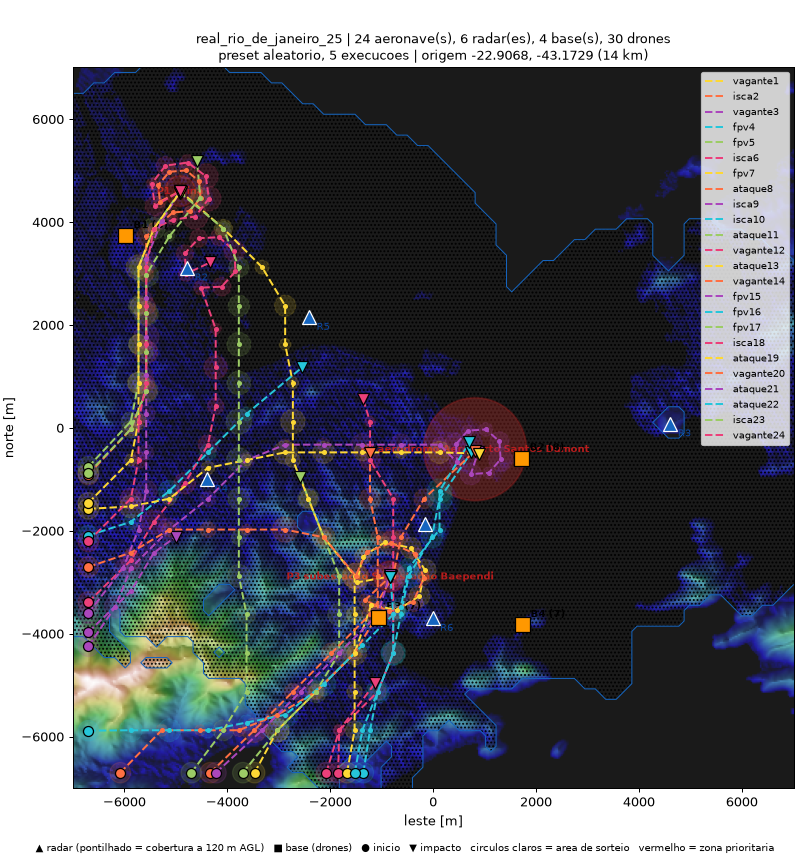
\includegraphics[width=0.75\textwidth]{figs/cenario_realista.png}
\caption{Missão de teste no Rio de Janeiro com composição equilibrada: 24 ameaças (6 de cada classe) entrando pelo setor
sudoeste, em rotas tracejadas que seguem o relevo e terminam nos impactos ($\blacktriangledown$); as munições vagantes
orbitam os alvos antes de mergulhar. Três ativos defendidos (vermelho), entre eles o aeroporto Santos Dumont; seis
radares nos morros ($\blacktriangle$, com a cobertura a 120~m sobre o terreno em pontilhado) e quatro bases com 30
interceptadores ($\blacksquare$).}
\label{fig:cenario}
\end{figure}

% =====================================================================================================
\section{Protocolo experimental}\label{sec:protocolo}

\paragraph{Sementes pareadas.} Uma \conceito{semente} é o número que inicializa o gerador de números aleatórios; com a
mesma semente, os mesmos sorteios se repetem. A execução $k$ de cada missão usa a mesma semente para todos os métodos, de
modo que todos enfrentam exatamente as mesmas rotas, velocidades, manobras, medidas de radar, falsos alarmes e iscas. As
diferenças entre métodos, portanto, não vêm de sorteios diferentes, e a comparação pode ser feita par a par.

\paragraph{O que é avaliado.} Os métodos sem parâmetros ajustados a partir de dados (M1--M22) são avaliados nas 192
missões, com 5 execuções cada (960 episódios por método). A árvore com utilidade (M23) é ajustada nas missões de treino
e avaliada em todas. As redes (M24--M29) são treinadas nas 128 missões de treino e avaliadas nas 64 de teste (320
episódios), para cada uma das 3 sementes de treino. As ablações usam 3 execuções por missão.

\paragraph{Métricas.} A métrica principal é o dano normalizado $D$~\eqref{eq:dano}; reportamos também o custo
$C$~\eqref{eq:custo_ep}, que soma ao dano a penalidade dos interceptadores desperdiçados, a fração das ameaças armadas
interceptadas, o número de impactos em zonas prioritárias, os interceptadores desperdiçados e gastos por ameaça e o tempo
de decisão.

\paragraph{Intervalos de confiança.} Reportamos a média de cada métrica com um \conceito{intervalo de confiança} de
95\,\%, a faixa que, com 95\,\% de confiança, contém o valor médio verdadeiro. Ele é obtido por
\conceito{\emph{bootstrap}}: reamostra-se o conjunto de dados com reposição milhares de vezes, recalcula-se a média em
cada reamostra e tomam-se os percentis de 2,5 e 97,5\,\%. Reamostramos \emph{missões}, e não episódios, porque episódios
da mesma missão são parecidos entre si; tratá-los como independentes produziria intervalos estreitos demais.

\paragraph{Testes de significância.} Para decidir se um método é melhor que a referência (o húngaro ponderado, M7), usamos o
\conceito{teste de Wilcoxon pareado}: para cada par (missão, semente), calcula-se a diferença de dano entre os dois métodos,
e o teste verifica se essas diferenças tendem a um lado mais do que o acaso explicaria, sem supor que sigam uma
distribuição normal. Reportamos o valor $p$: a probabilidade de observar diferenças tão sistemáticas se os dois métodos
fossem, na verdade, equivalentes. Para as redes, cada par usa a média sobre as sementes de treino.

\paragraph{Custo computacional.} O tempo de decisão é medido por chamada, com um processo por episódio.
\todo{processador da máquina em que o benchmark rodar.}

% =====================================================================================================
\section{Resultados}\label{sec:resultados}

\subsection{Validação das implementações}\label{sec:validacao}
Antes de comparar desempenho, é preciso confirmar que as implementações estão corretas. Uma forma objetiva de fazê-lo é
usar as equivalências que a teoria garante: certos pares de algoritmos, embora funcionem de modo diferente, devem chegar
à mesma solução. Em 320 rodadas de decisão de 8 cenários, todos os algoritmos resolveram exatamente a mesma instância
(Tabela~\ref{tab:equivalencia}).

Os três pares teoricamente equivalentes --- leilão e húngaro ponderado (M9 e M7, mesmo problema de atribuição), CBAA com
grafo completo e guloso global (M11 e M10) e MILP e húngaro sobre o WTA (M15 e M14, mesmo problema linear) --- atingem o
mesmo valor do objetivo em 100\,\% das rodadas. A designação coincide em 99,6, 100 e 96,8\,\% dos interceptadores,
respectivamente; as diferenças vêm de soluções alternativas com o mesmo valor (empates), e não de erros.

Entre os métodos que otimizam o valor esperado~\eqref{eq:F}, o MMR fica em média a 0,1\,\% do melhor valor encontrado
na rodada, mas chega a ficar 7,6\,\% abaixo em algumas; a busca local é a que mais se aproxima do melhor (99,99\,\% em
média, pior caso 98,6\,\%). O custo varia em duas ordens de grandeza: atribuição, leilão, MMR e busca local resolvem uma
rodada em 4 a 6~ms (mediana), o MILP em 16~ms, o algoritmo genético em 93~ms, o recozimento simulado em 234~ms e a colônia
de formigas em 487~ms.

\inp{tabelas/equivalencia}

\subsection{Escolha da guiagem terminal}\label{sec:res_guiagem}
A guiagem é um componente fixo do benchmark, mas precisa ser escolhida. Um experimento 1$\times$1 --- um interceptador
contra uma aeronave, 300 encontros por combinação, os mesmos para todas as leis --- comparou leis de guiagem contra cada
perfil evasivo (Tabela~\ref{tab:guiagem}), com dois objetivos: fixar a lei usada no benchmark e medir a probabilidade
$P_T$ de contato na primeira passagem, usada no modelo de sucesso~\eqref{eq:q}. A navegação proporcional com constante
$N'=4$ teve a maior taxa de contato na primeira passagem contra as manobras não reativas, e é a lei usada; sua taxa média
de contato na primeira passagem, 0,85, é o valor de $P_T$.
A guiagem preditiva (MPC), que supõe velocidade constante do alvo ao longo do horizonte, ficou abaixo da navegação
proporcional contra as manobras (por exemplo, 71 contra 88\,\% de contato na primeira passagem contra zigue-zague, com
30~m/s$^2$) e custou ordens de grandeza mais tempo por passo --- um primeiro indício, no nível de um único encontro, de
que a hipótese de velocidade constante é frágil diante de alvos evasivos.

\inp{tabelas/guiagem}

\subsection{Comparação dos métodos de alocação}\label{sec:res_alocacao}
\todo{comentar as tabelas principais (teste e treino): ranking por dano e por custo, quem desperdiça interceptadores em
iscas, significância contra M7.}

\inp{tabelas/principal_teste}
\inp{tabelas/principal_treino}

\subsection{Efeito da composição do enxame, da cidade e da escala}\label{sec:res_perfil}
\todo{comentar: quais métodos sofrem mais com a saturação por iscas (desperdício) e com a composição tática (FPV e
munições vagantes, lentas e baixas); diferença entre cidades de treino e de teste; crescimento do dano com $N$.}

\inp{tabelas/composicao}
\inp{tabelas/cidade}
\inp{tabelas/tamanho}
\IfFileExists{figs/dano_vs_n.pdf}{\begin{figure}[t]\centering\includegraphics[width=\columnwidth]{figs/dano_vs_n.pdf}
\caption{Dano médio nas missões de teste em função do número de ameaças.}\label{fig:dano_n}\end{figure}}{}

\subsection{Ablações: troca de alvo, salvas, comunicação e guiagem}\label{sec:res_ablacao}
Uma \conceito{ablação} remove ou altera um componente de um método para medir quanto ele contribui.
\todo{comentar.}

\inp{tabelas/ablacao}

\subsection{Métodos aprendidos}\label{sec:res_redes}
\todo{comentar imitação, PPO do zero e refinado, DeepSets $\times$ atenção, variância entre sementes, generalização.}

% =====================================================================================================
\section{Discussão}\label{sec:discussao}
\todo{síntese por família; efeito das iscas e do desperdício (dano $\times$ custo); efeito da composição e do voo
baixo sobre a previsão de velocidade constante; generalização para cidades nunca vistas; custo computacional e
escalabilidade; recomendações.}

\subsection{Limitações}
\begin{itemize}
  \item \textbf{Modelo de interceptador.} Os interceptadores são pontos de massa em duas dimensões, com velocidade
        constante e aceleração lateral limitada; não há dinâmica de atitude nem vento sobre eles. Por isso, a altura da
        ameaça afeta a detecção pelo radar, mas não o engajamento.
  \item \textbf{Modelo de ameaça.} A velocidade de cada ameaça é constante ao longo da rota (o aumento de velocidade da
        munição vagante no mergulho não é modelado), e só o trecho final das rotas de longo alcance, dentro de um mapa de
        12 a 14~km, é simulado. A seção radar, o valor de dano de cada classe e a penalidade por desperdício
        ($\eta=0{,}2$) são hipóteses do modelo; os parâmetros de fontes abertas vêm de reportagens e análises
        secundárias, não de especificações oficiais.
  \item \textbf{Ativos.} Os alvos dependem do mapeamento colaborativo do OpenStreetMap, cuja cobertura varia entre as
        cidades; a importância de cada categoria de ativo é uma escolha do modelo.
  \item \textbf{Sensor próprio ideal.} Na fase final, o interceptador vê a aeronave sem erro.
  \item \textbf{Adaptações.} As técnicas foram adaptadas a interceptadores descartáveis de contato único. A árvore com
        utilidade (M23) perde o ramo de reforço, e o MILP (M15) representa só a parte de alocação de~\cite{cruz2025}, sem
        obstáculos nem bateria. Só as redes treinadas por reforço conhecem a penalidade por desperdício; os métodos de
        WTA usam o seu próprio custo de lançamento, e os demais não têm nenhum.
  \item \textbf{Modelo de sucesso.} Os métodos M13--M20 dependem de~\eqref{eq:q}, calibrado num experimento 1$\times$1; um
        modelo melhor poderia favorecer essa família.
  \item \textbf{Orçamento de treino.} As redes foram treinadas com um orçamento fixo e modesto; resultados com mais
        treino podem diferir.
\end{itemize}

\section{Conclusão}\label{sec:conclusao}
\todo{}

\section*{Disponibilidade de código e dados}
O simulador, os geradores de missões, a extração dos ativos do OpenStreetMap, as 192 missões, as implementações dos 29
métodos (um arquivo por método), os modelos treinados e os scripts que geram as tabelas e figuras deste artigo estão
disponíveis em \todo{repositório}. Qualquer método pode ser rodado isoladamente sobre qualquer missão
(\texttt{rodar.py}).


\bibliographystyle{unsrtnat-pt}
\bibliography{refs}
\end{document}
